\setcounter{chapter}{4} % previous chapter number

\chapter{Dynamical systems}
\label{h:dynamical}

\begin{quote}
The mathematician's patterns, like the painter's or the poet's must be beautiful; the ideas, like the colours or the words must fit together in a harmonious way. Beauty is the first test.

--- Godfrey H. Hardy
\end{quote}

\begin{quote}
As for everything else, so for a mathematical theory: beauty can be perceived but not explained.

--- Arthur Cayley
\end{quote}

%\setcounter{page}{1}
\minitoc

In this chapter, we will study some aspects of the dynamics of nonlinear systems. We will see that these systems can exhibit wonderfully complex and intricate phenomena, producing both pretty pictures and profound insights into the behaviour of physical processes.

After an example from the photonics world, we will look at 1D discrete systems. 2D discrete systems are studied next, and finally we will discuss continuous systems, i.e. systems that are described by differential equations instead of difference equations.

\section{Chaos in a photonic system}

\begin{figure}
\centering
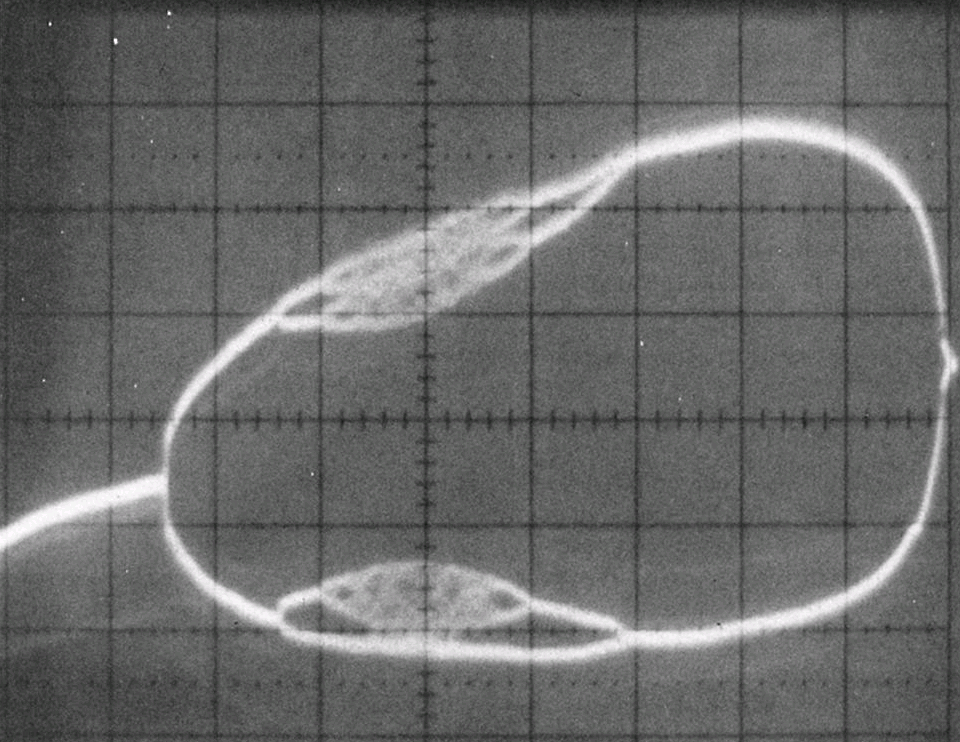
\includegraphics[width=8cm]{dynamic/figures/CO2_chaos}
\caption{Laser intensity as a function of modulator bias in a CO$_2$--laser.}
\label{fig-co2}
\end{figure}

In 1991, scientists at the University of Lille studied a CO$_2$--laser which contained an electrooptic absorber inside the cavity to modulate the output intensity of the laser beam. An alternating current $I(t)=A+B \cos (\omega t)$ was applied to the modulator. The modulation amplitude $B$ was kept fixed at 3V, and the modulator frequency $\omega$ was set to 640 kHz, a resonance frequency of the laser. Next, the experimenters varied the DC bias $A$ from 60V to 460V and observed what happened to the laser output. They sampled the output 640 000 times per second, i.e. in lockstep with the modulation frequency. They did this experiment for various values of the DC bias to produce the oscilloscope picture of Fig.~\ref{fig-co2}.

For low values of the DC offset, there is only a single branch, meaning that the laser intensity varies with the same frequency as the modulation current, which is just what you would expect. However, for larger DC offsets, there are suddenly two branches in the curves: the laser oscillation takes two periods of the modulation to repeat. This pattern with doubled period is called a \emph{subharmonic} of the modulation period. Increasing the DC offset even further leads to patterns which take 4, 8 or more modulation periods to repeat. There is even a certain range where the laser output varies between so many levels that it looks very chaotic.

The combination of CO$_2$--laser plus absorber can be described by a set of relatively simple nonlinear rate equations (see e.g. the course 'High speed photonic components'). At first sight, it is very surprising that dynamical systems which are described by relatively simple--looking differential equations can exhibit such rich behaviour.

In this chapter, we will study some aspects of this complex behaviour of dynamical systems, starting from very simple 1D models described by difference equations. Higher dimensional systems and systems described by differential equations instead of difference equations will also be treated.

\section{1D discrete systems}

\subsection{Dynamical systems}

A \emph{dynamical system} consists of a set of possible states, together with a rule that determines the present state in terms of the past states. E.g., a simple model for growth of bacteria in a lab culture is that the population doubles each hour. So, the update rule of this system is

\begin{equation}
x_n = f(x_{n-1}) = 2 x_{n-1} \label{eq-exp-growth}
\end{equation}

 Here, the state $x$ designates the population size, and the subscript $n$ stands for the state at time step $n$, in this case the state after $n$ hours.  

Based on the properties of the update rule, we can distinguish several types of dynamical systems.

Here, we require the rule to be \emph{deterministic}, which means we can determine the present state uniquely from the past states.

If the update rule is applied at discrete times, the system is called a \emph{discrete--time} system. In the limit of infinitesimally small time steps, the governing rules become a set of differential equations, and we end up with a \emph{continuous--time} system.

\subsection{1D maps}

A function $f$ whose input and output space are the same is called a \emph{map}. The evolution of a dynamical system is governed by multiple applications of the update rule $f$. Let us define $f^2(x)=f(f(x))$ and more generally define $f^k(x)$ as the results of applying $f$ to $x$ $k$ times. The set of points ${x_0, f(x_0), f^2(x_0), ...}$ is called the \emph{orbit} of $x_0$ under $f$. The starting point $x_0$ is called the \emph{initial value} of the orbit.

Of interest in the study of dynamical systems is the limiting behaviour of $f^k(x)$ for large values of $k$. For the exponential growth scenario of Eq.~\ref{eq-exp-growth}, the population will clearly increase without bound, which is obviously not a realistic model. As you will show in the next exercise, an improved model might be given by

\begin{equation}
f(x) = 2 x (1-x) \label{eq-logistic-growth}
\end{equation} 

Here, the population size is normalised to lie between 0 and 1. Contrary to the exponential growth model, this so--called \emph{logistic growth} model has a nonlinear update rule.

\begin{sidebar}
\begin{ex}
Show by using a calculator or a computer that populations evolving under the rule $f(x) = 2 x (1-x)$ tend to the population of 0.5 as time evolves. Do this for several initial values. You will find the size $x=0.5$ eventually 'attracts' any of these starting populations.
\end{ex}
\end{sidebar}

\subsection{Cobweb plots}

A cobweb plot is a graphical representation of the orbit of an initial value under a 1D map. It is obtained by drawing the graph of the update rule, together with the diagonal $y=x$ (see Fig.~\ref{fig-cobweb1}).

\begin{figure}
\centering
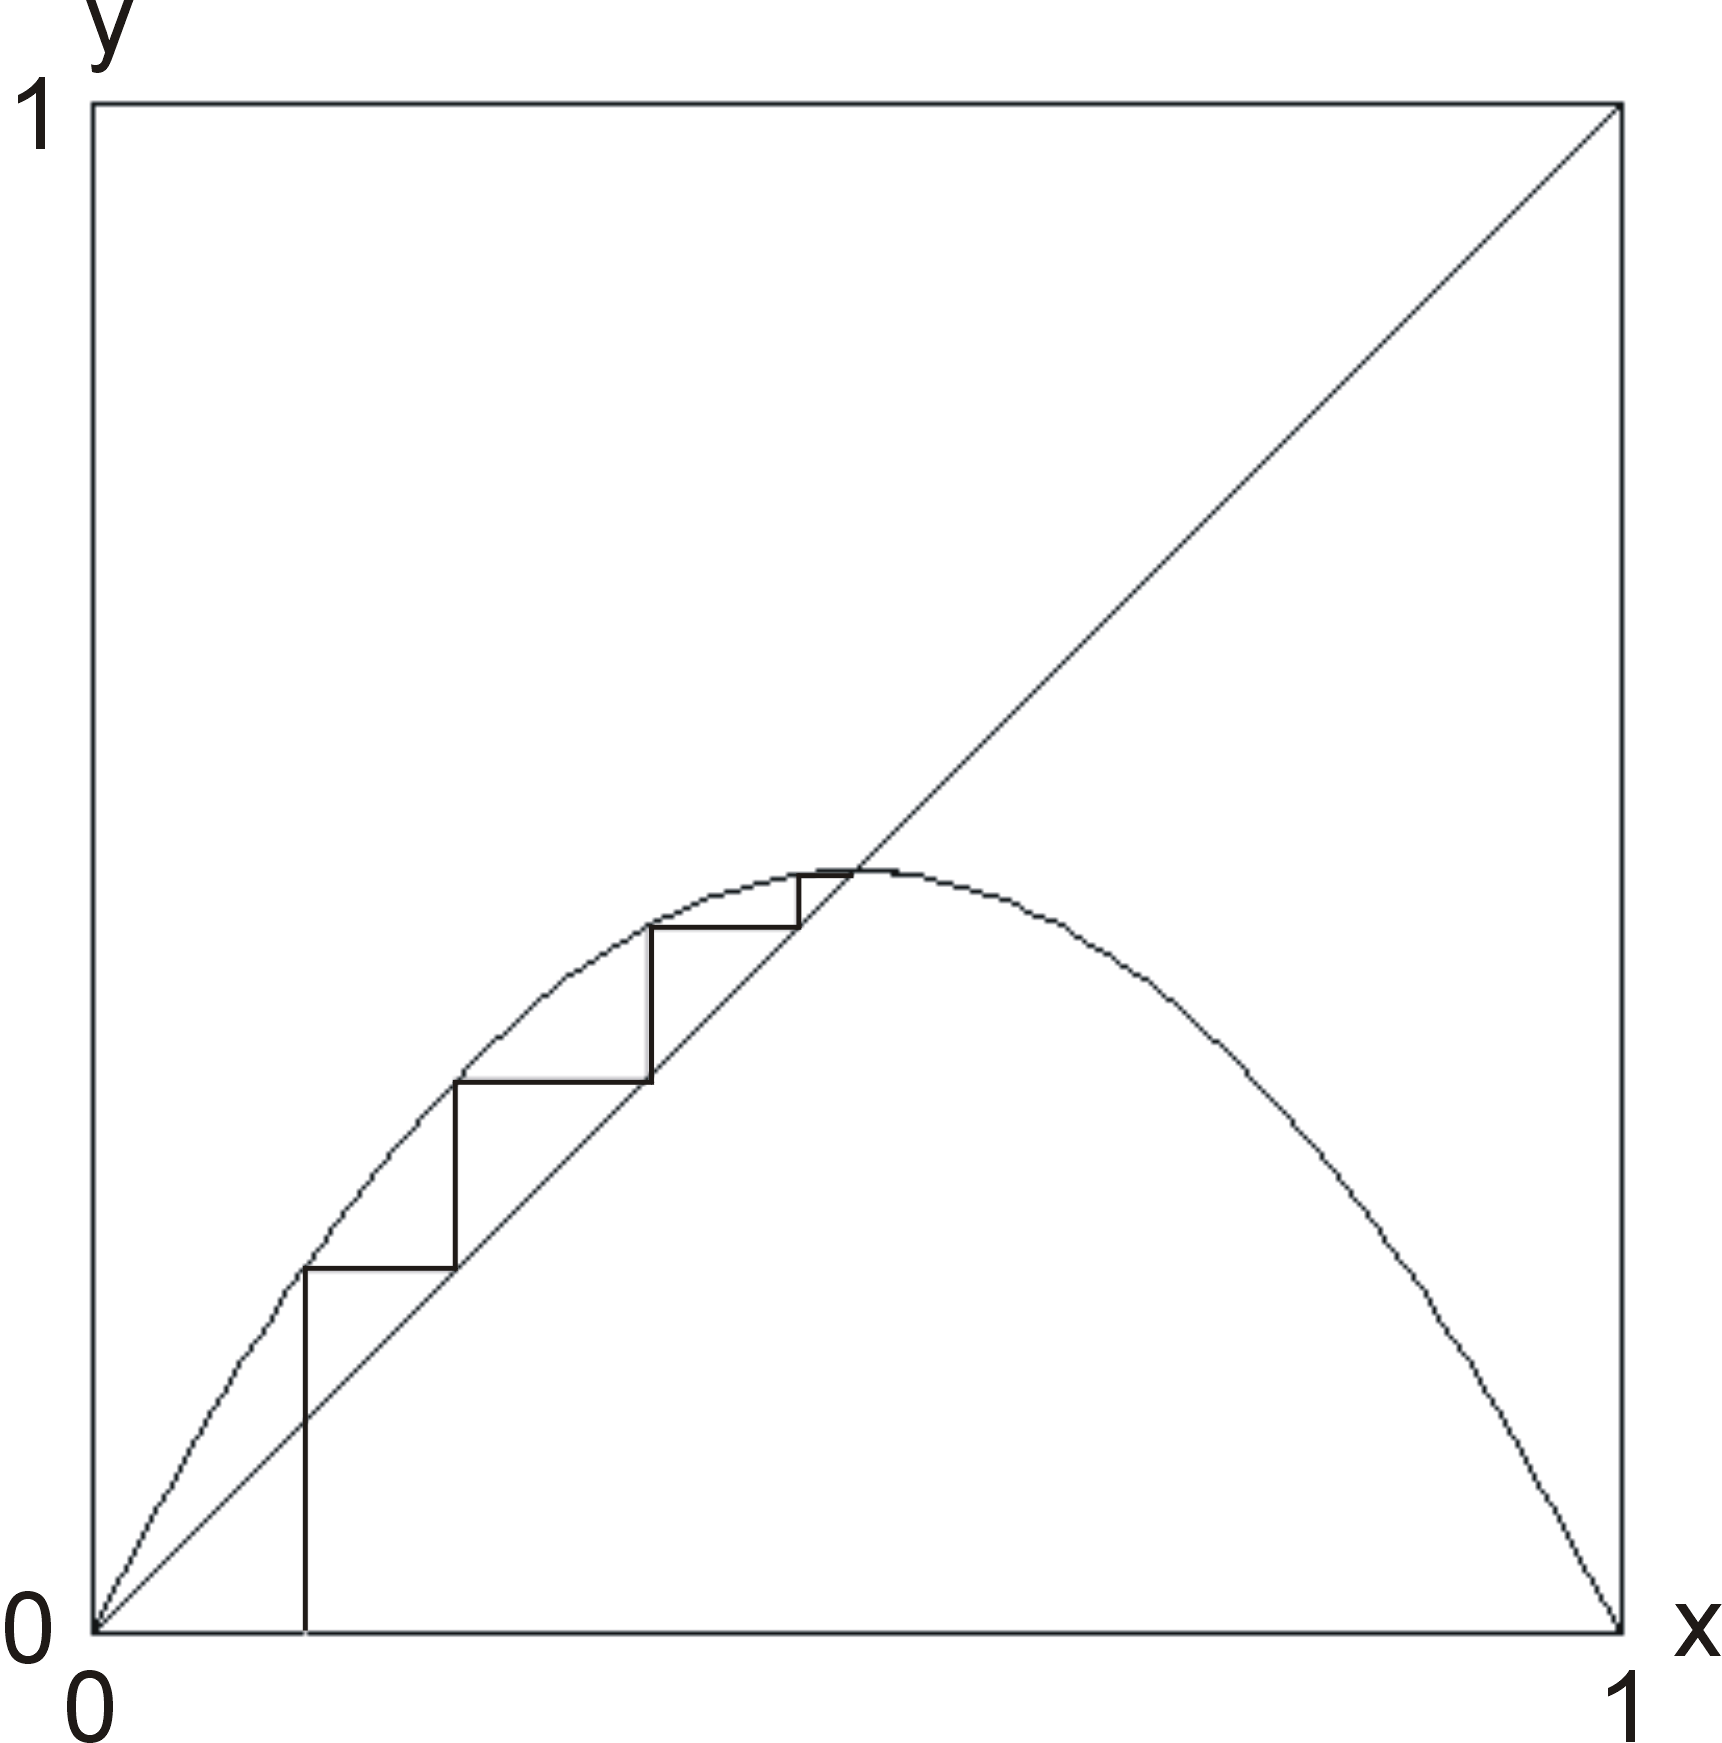
\includegraphics[width=7cm]{dynamic/figures/cobweb1}
\caption{Cobweb plot for $f(x)=2x(1-x)$.}
\label{fig-cobweb1}
\end{figure} 

Sketching the orbit of an initial point is done as follows. E.g., starting with the input value $x_0=0.1$ and $f(x)=2x(1-x)$ in Fig.~\ref{fig-cobweb1}, we can easily plot $f(0.1)$ by drawing a vertical line starting from $x_0=0.1$ to the curve $f(x)$, which gives us a value of $0.18$. Next, we need to turn this output value of $0.18$ to an input value to compute $f(0.18)$. This is done by drawing a horizontal line from the input--output pair $(0.1,0.18)$ until it reaches the diagonal $y=x$. Now, the process can be repeated by drawing a sequence of vertical and horizontal line segments between the curve of the update rule and the diagonal.

From the cobweb plot, it is clear that the orbit will converge to the point $x=0.5$, which lies on the intersection of the graph of the update function and the diagonal.

Such points where $f(x)=x$ are called \emph{fixed points}. They are of extreme importance when studying the dynamics of a system, as they contain information on the asymptotic behaviour of the system.

\begin{sidebar}
\begin{ex}
Let $f$ be the map given by $f(x) = (3x-x^3)/2$. Draw cobweb plots for orbits with initial values $x=1.6$ and $x=1.8$. Calculate the fixed points of this map. What happens with orbits starting out in the vicinity of each of these fixed points?
\end{ex}
\end{sidebar}

\subsection{Stability of fixed points}

Not all fixed points are alike. A \emph{stable} fixed point has the property that points near it will move even closer to it as the dynamical system evolves. For an \emph{unstable} fixed point, the opposite is true: points starting out in its neighbourhood will rapidly move away as time progresses.

A good analogy is that a ball at the bottom of a valley is stable, while a ball balanced at the tip of mountain will be unstable.

Stability is an important concept as real--world systems are constantly subjected to small perturbations. Therefore, a steady state observed in a real system must correspond to a stable fixed point. If the fixed point were unstable, small perturbations would move the orbit away from the fixed point, which would then be not observed.

A stable, attracting fixed point is often called a \emph{sink}, while an unstable, repelling fixed point is called a \emph{source}.

To formulate this more precisely, let's first introduce the concept of an \emph{epsilon neighbourhood} $N_\epsilon(p)$, which is the set of all real numbers within a distance $\epsilon$ of $p$:

\begin{equation}
N_\epsilon(p) = \{x \in \mathbb{R} ; |x-p| < \epsilon\}
\end{equation} 

A fixed point is called a sink if there exists an $\epsilon > 0$ such that for all points $x$ in the epsilon neighbourhood $N_\epsilon(p)$, $\lim_{k \to \infty} f^k(x) = p$.

Similarly, a fixed point is called a source if there is an epsilon neighbourhood $N_\epsilon(p)$ such that each $x$ in $N_\epsilon(p)$ except $p$ eventually maps outside of $N_\epsilon(p)$.

How can we determine from the shape of $f$ whether a fixed point is a source or a sink? The answer lies in the following theorem:

\begin{thm}
\label{th-stab-fix}
Let $f$ be a smooth map of $\mathbb{R}$ with fixed point $p$. 
\begin{enumerate}
\item
If $|f'(p)| < 1$, then $p$ is a sink.
\item 
If $|f'(p)| > 1$, then $p$ is a source. 
\end{enumerate}
\end{thm} 

We only prove the first part, as the second is completely analogous.

From the definition of the derivative, we get (for points $x \ne p$)

\begin{equation}
\lim_{x \to p} \frac{\left|f(x)-f(p)\right|}{|x-p|} = \left|f'(p)\right|
\end{equation} 

Since $|f'(p)| < 1$ there is number $a$ between $|f'(p)|$ and 1. This means that there must be a neighbourhood $N_\epsilon(p)$ where

\begin{equation}
\frac{\left|f(x)-f(p)\right|}{|x-p|} < a, \hspace{.5cm} \forall x \in N_\epsilon(p)
\end{equation}

Using the fact that $p$ is a fixed point, we get

\begin{equation}
\left|f(x)-p\right| < a |x-p|,  \hspace{.5cm} \forall x \in N_\epsilon(p) \label{eq-stab-fix}
\end{equation}

So, $f(x)$ is closer to $p$ than $x$ was to $p$ by at least a factor of $a$, meaning that $f(x)$ is also in $N_\epsilon(p)$.

Let's rewrite Eq.~\ref{eq-stab-fix} slightly:

\begin{equation}
\left|f^1(x)-p\right| < a \left|f^0(x)-p\right|,  \hspace{.5cm} \forall x \in N_\epsilon(p)
\end{equation} 

Since $f^1(x)$ is also in $N_\epsilon(p)$, we can repeat the above procedure to get

\begin{equation}
\left|f^k(x)-p\right| < a\left|f^{k-1}(x)-p\right| < a^2\left|f^{k-2}(x)-p\right|< ... < a^k |x-p| 
\end{equation}  

Since $a<1$, we get eventually that

\begin{equation}
\lim_{k \to \infty} \left|f^k(x)-p\right| = 0
\end{equation} 

This proves that $p$ is a sink.

The set of initial conditions that is attracted to the sink is called the \emph{basin} of the sink. From the proof of Theorem~\ref{th-stab-fix}, we get that the basin of a sink contains at least a small epsilon neighbourhood, but in practise sinks often attract a large set of initial conditions.

Finally, note that Theorem~\ref{th-stab-fix} does not say anything about the case $|f'(p)|=1$.

\begin{sidebar}
\begin{ex}
Discuss the stability of the fixed points of the map $f(x) = (3x-x^3)/2$.
\end{ex}
\end{sidebar}

\begin{sidebar}
\begin{ex}
Discuss the stability of the fixed points of the map $f(x) = x^3 + x$.
\end{ex}
\end{sidebar}

\subsection{Periodic points}

If we change the proportionality constant $a$ of the logistic map $f_a(x)=ax(1-x)$ to 3.3, we get a different behaviour than what we have seen so far. The fixed points are $x=0$ and $x=23/33$, both of which are unstable. So, without any fixed points to attract them, where do the orbits go? Using a calculator or a computer, it is easy to show that the orbit settles into a pair of alternating values $p_1=0.4794$ and $p_2=0.8236$. Fig.~\ref{fig-cobweb2} plots the cobweb diagram for this case.

\begin{figure}
\centering
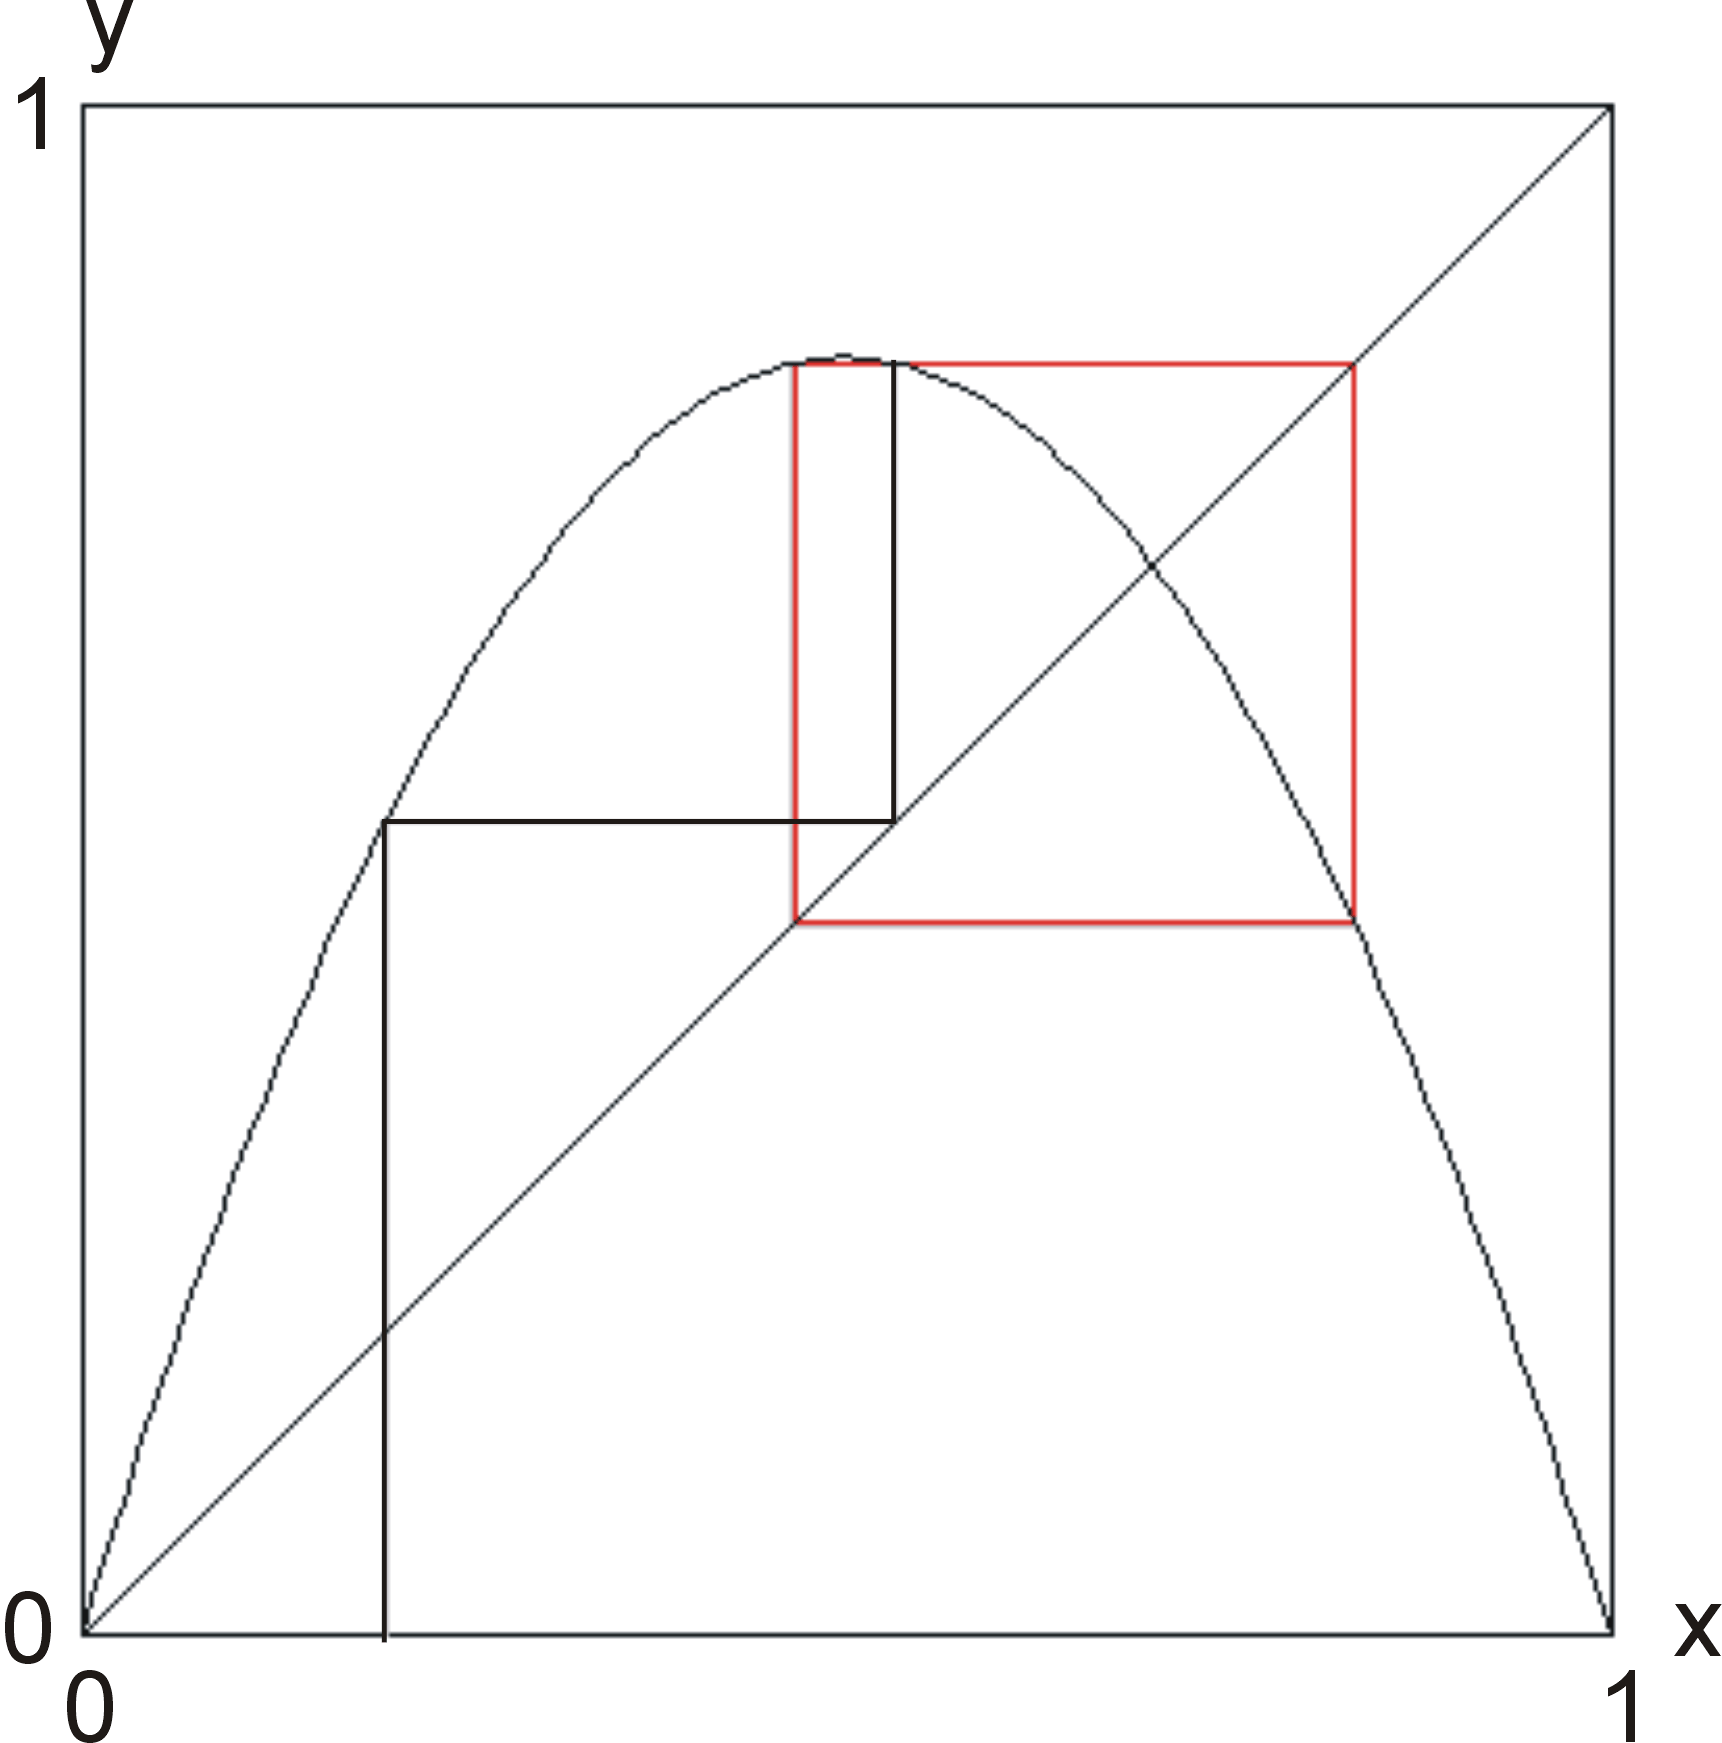
\includegraphics[width=7cm]{dynamic/figures/cobweb2}
\caption{Cobweb plot for $f(x)=3.3x(1-x)$.}
\label{fig-cobweb2}
\end{figure} 

Note that $f(p_1)=p_2$ and $f(p_2)=p_1$. Another way of looking at this it saying that $f^2(p_1)=p_1$, so $p_1$ is a fixed point of $h=f^2$ (the same is obviously true for $p_2$).

More formally, we call $p$ a \emph{periodic point of period $k$} (or period--$k$ point) of a map $f$ if $f^k(p)=p$ and $k$ is the smallest positive integer for which this is true.

Note that this definition does not imply that any fixed point of $f^k$ is a period--$k$ point of $f$, as there might be a smaller integer $n$ for which $f^n(p)=p$.

Just like fixed points, period--$k$ orbits can be attracting (sinks) or repelling (sources). To discuss the stability, we apply Theorem~\ref{th-stab-fix} on the map $f^k$, because a period--$k$ point is a fixed point of $f^k$.

For a period--2 point, we need to evaluate $|f^2(p_1)|$, which can be done easily with the chain rule:

\begin{equation}
|f^{2'}(p_1)| = |f'(f(p_1)) f'(p_1)| = |f'(p_2) f'(p_1)|
\end{equation}  

This can be easily generalised to period--$k$ points:

\begin{sidebar}
\begin{ex}
Show that the following holds: a periodic orbit $\{p_1, p_2, ..., p_k\}$ is a sink if

$$|f'(p_1) f'(p_2) ... f'(p_k)| < 1$$

and a source if

$$|f'(p_1) f'(p_2) ... f'(p_k)| > 1$$

\end{ex}
\end{sidebar}

Note that stability is a collective property of the periodic orbit, in the sense that $f^{k'}(p_i) = f^{k'}(p_j)$ for all values of $i$ and $j$.

\begin{sidebar}
\begin{ex}
% Chaos - Alligood T1.5
Verify that the map $f(x)=2x^2-5x$ has fixed points at 0 at 3. Use this information to more easily find a period-2 orbit for $f$, without needing to solve for the zeroes of a fourth-order polynomial.
\end{ex}
\end{sidebar}


\subsection{The family of logistic maps}

We have already seen that the scaling parameter $a$ in the family of logistic maps $f_a(x)=ax(1-x)$ can have a large influence on the behaviour of the system: for some ranges of $a$ there is only one attracting solution, for other ranges there is a stable period--2 orbit.

\begin{figure}
\centering
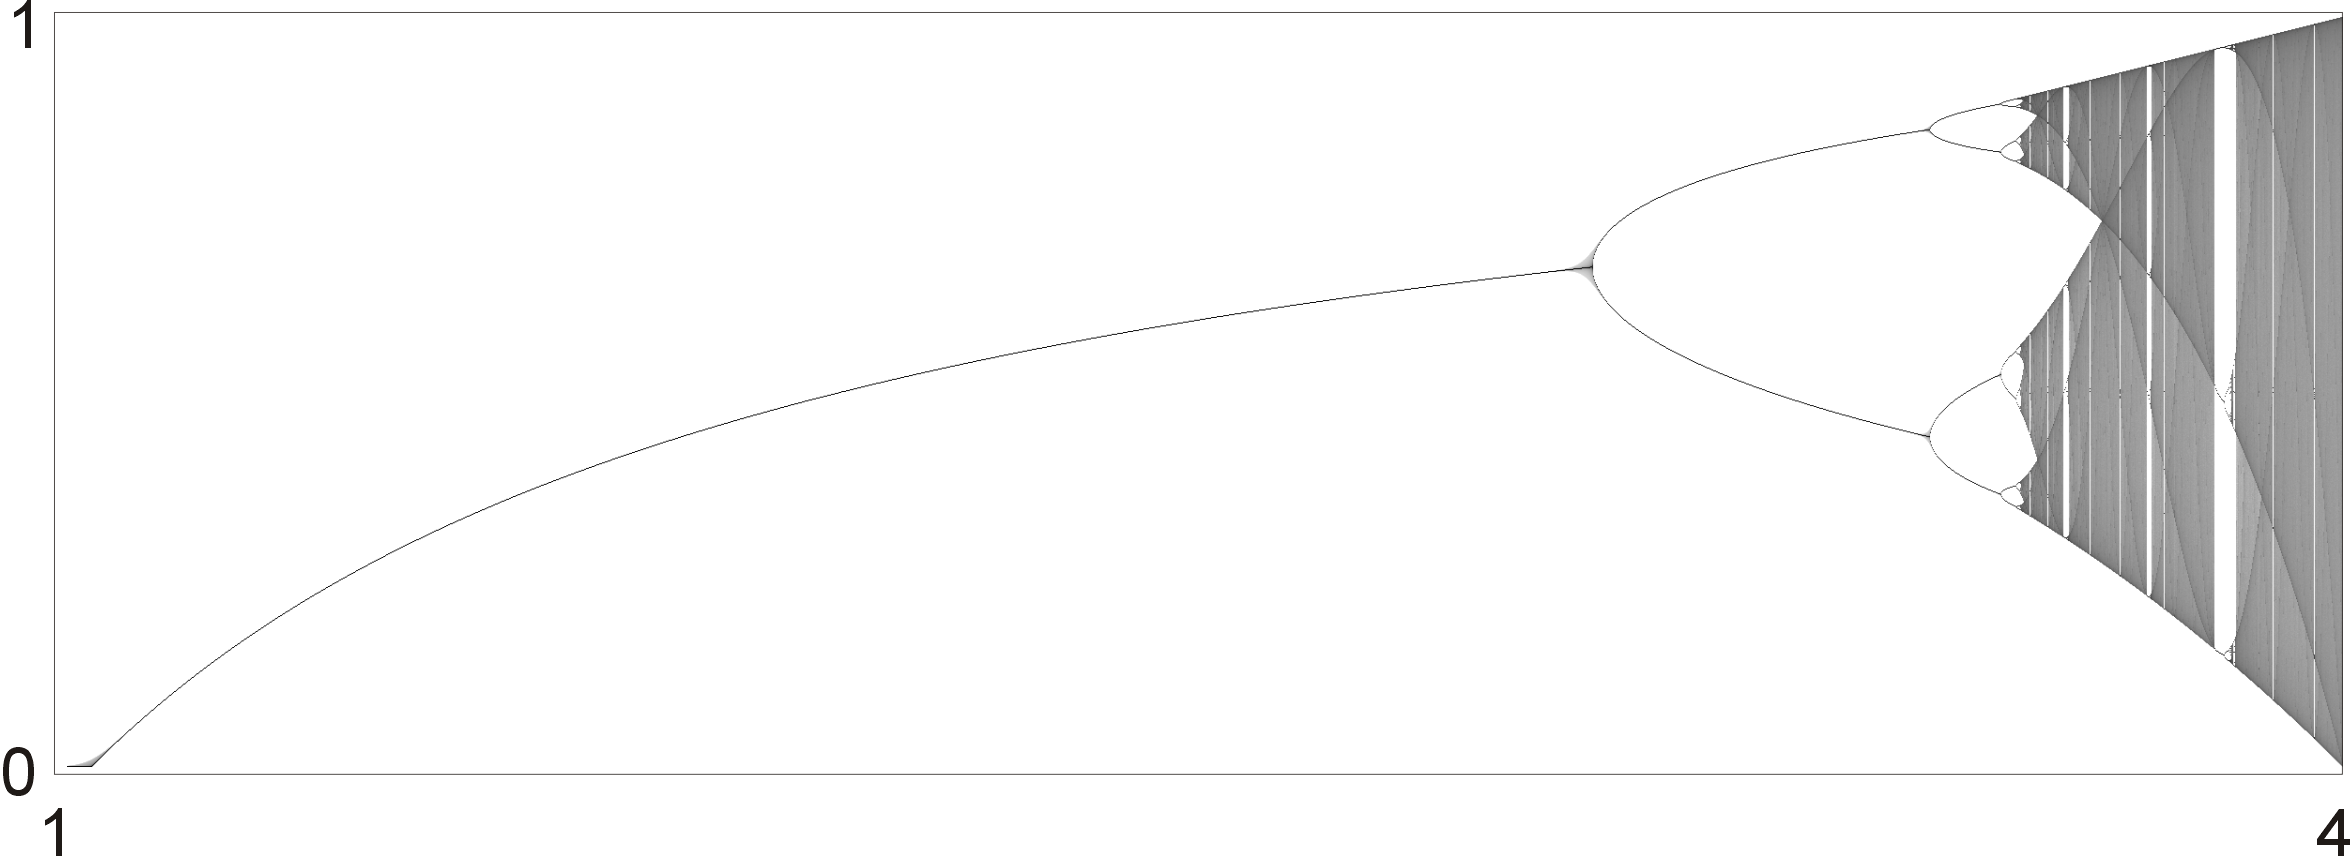
\includegraphics[width=15cm]{dynamic/figures/bifurcation}
\caption{Bifurcation diagram for the family of logistic maps for $f(x)=ax(1-x)$.}
\label{fig-bifur}
\end{figure} 

To visualise the behaviour of the logistic map for various values of $a$ we can make a diagram like the one in Fig.~\ref{fig-bifur}. On the horizontal axis we plot $a$, while the vertical axis shows $x$--values. The figure is constructed as follows: for each $a$--value, pick a random starting value $x$, and calculate its orbit under the map $f_a(x)$. Discard the first 100 points of this orbit, and plot the remaining points of the orbit. Then increment $a$ and start the procedure again. The points that are plotted will (within the resolution of the picture) approximate either fixed or periodic sinks or other attracting orbits of the dynamic system \footnote{One might ask how Fig.~\ref{fig-bifur} will change if different starting values of $x$ were selected. Surprisingly, for the logistic map nothing will change, which indicates that for each $a$ value, there is at most one attracting orbit.}.

Fig.~\ref{fig-bifur} (and also Fig.~\ref{fig-co2}) is called a \emph{bifurcation diagram} and shows the birth, evolution and death of attracting orbits. The term 'bifurcation' is used to describe significant changes in the set of attractors in a dynamical system. E.g. at $a=3$, there is a transition between a single sink and the emergence of a period--2 point. This type of bifurcation is called a \emph{period--doubling bifurcation} or also (because of its characteristic shape) a \emph{pitchfork bifurcation}. For $a$ slightly larger than 3.45, there appears to be a period--4 sink. In fact, there is an entire sequence of periodic sinks, one for each period 2, 4, 8, 16, 32,... . Such a sequence is called a \emph{period--doubling cascade}.

\begin{sidebar}
\begin{ex}
Write a computer program that finds the $a$--values at which the bifurcations occur in the period--doubling cascade 2, 4, 8, 16, ... . Call the sequence of these values $a_n$, and calculate

$$\frac{a_{n-1} - a_{n-2}}{a_{n} - a_{n-1}}$$

What do you observe as $n$ tends towards infinity? Repeat the experiment for the period--3 cascade: 3, 6, 12,... . Also experiment with a different nonlinear map, like $f_a(x)=a-x^2$.

The number 4.669201609 is called \emph{Feigenbaum's constant}.
\end{ex}
\end{sidebar}

For other values of the parameter $a$, the orbit appears to randomly fill out the interval $[0,1]$, or a subinterval. A typical cobweb plot for such a situation is shown in Fig.~\ref{fig-cobweb3}. These non--periodic attracting sets are called \emph{chaotic attractors} and are obviously much harder to describe than periodic sinks.

\begin{figure}
\centering
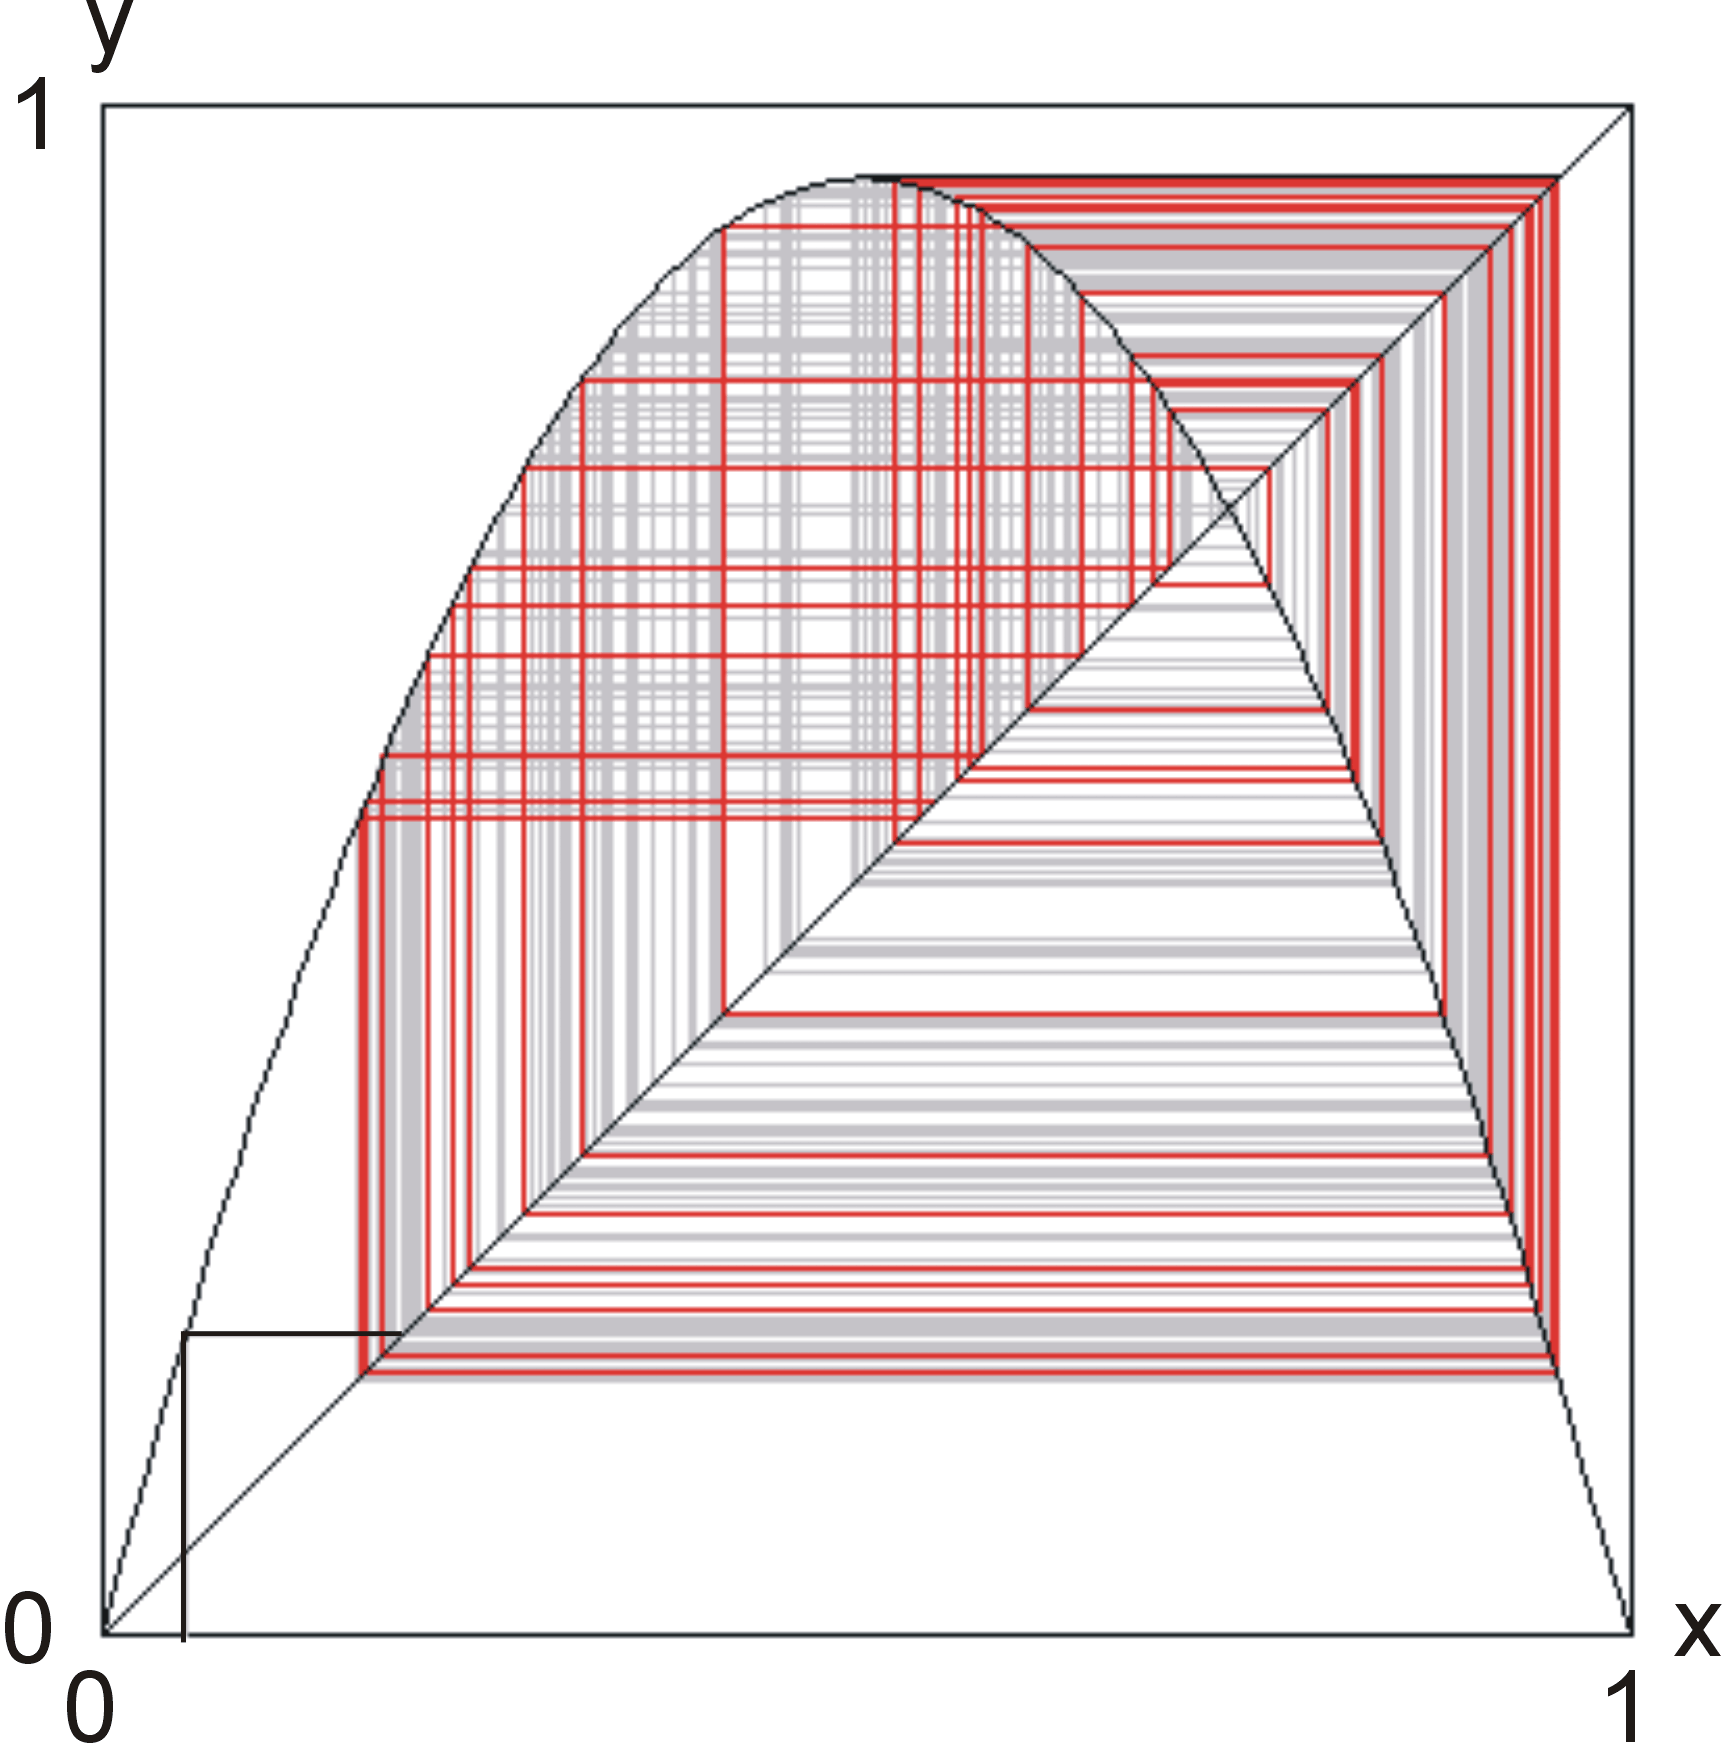
\includegraphics[width=7cm]{dynamic/figures/cobweb3}
\caption{Cobweb plot for the logistic map in the case of a chaotic attractor.}
\label{fig-cobweb3}
\end{figure} 

So are these non--periodic attractors what we mean by 'chaos'? Partly. Another important concept in that regard is the sensitive dependence on initial conditions, which we will explore next.

\subsection{Sensitive dependence on initial conditions}

\begin{table}
\centering
\begin{tabular}{|c|c|c|}
\hline
${\bf n}$  & ${\bf f_n(0.3)}$ & ${\bf f_n(0.301)}$  \\
\hline
0  & 0.3000 & 0.3010  \\
\hline
1  & 0.8400 & 0.8416 \\
\hline
2  & 0.5376 & 0.5332 \\
\hline
3  & 0.9943 & 0.9956 \\
\hline
4  & 0.0225 & 0.0176 \\
\hline
5  & 0.0879 & 0.0692 \\
\hline
6  & 0.3208 & 0.2576 \\
\hline
7  & 0.8716 & 0.7650 \\
\hline
8  & 0.4476 & 0.7190 \\
\hline
9 & 0.9890 & 0.8081 \\
\hline
10 & 0.0434 & 0.6202 \\
\hline
\end{tabular}
\caption{Comparison of orbits of nearly identical points under the map $f(x)=4x(1-x)$.}
\label{table-sens}
\end{table}

Table~\ref{table-sens} shows the orbits of two points 0.3000 and 0.3010 under the map $f(x)=4x(1-x)$. Although these points start out close together, they quickly diverge. In fact, no matter how close together we choose these two points, they will eventually move apart. This sensitive dependence on initial conditions has some far--reaching implications. If a dynamic system exhibits these chaotic properties, it means we can never hope to accurately predict the long--term behaviour of the system, even though it is governed by deterministic and well--known rules. Sensitive dependence on initial conditions means that small variations in the initial state of the system (e.g. due to measurement errors or finite numerical precision), will always get amplified to such a degree that it is impossible to make long--term predictions on the evolution of the system. This is the hallmark of \emph{chaos}.

To quantify how sensitive an orbit is to variations in initial conditions, we will now introduce the concept of Lyapunov numbers and Lyapunov exponents.

We already learnt that for fixed points, stability is heavily influenced by the derivative of the map. E.g., if $p$ is a fixed point and $f'(p)=a > 1$, then the orbit of a point near $p$ will move away at a multiplicative rate of approximately $a$ per iteration. This also means that the difference between two points will by amplified at the same rate. Starting from these observations, we generalise this to arbitrary orbits by defining the \emph{Lyapunov number} of an orbit $\{x_0, x_1, x_2, ... \}$ as

\begin{equation}
L(x_0) = \lim _{n \to \infty}\left(\left|f'(x_0)\right|...\left|f'(x_{n-1})\right|\right)^{\frac{1}{n}}
\end{equation} 

if this limit exists.

The \emph{Lyapunov exponent} is defined as the logarithm of the Lyapunov number:

\begin{equation}
h(x_0) = \ln L(x_0) = \lim _{n \to \infty}\frac{1}{n}\left(\ln\left|f'(x_0)\right| + ... + \ln\left|f'(x_{n-1)})\right|\right)
\end{equation} 

Note that $h$ exists if and only if $L$ exists and is non--zero.

E.g., if the Lyapunov number of an orbit is equal to 2, this means that on average the distance between the orbit of $x_0$ and a neighbouring orbit will double each iteration. So, an orbit is called a \emph{chaotic orbit} if its Lyapunov number is greater than 1 (or its Lyapunov exponent is positive). 

\begin{sidebar}
\begin{ex}
Write a computer program to calculate the Lyapunov exponents for the family of logistic maps $f_a(x)=ax(1-x)$. Plot the Lyapunov exponent as a function of $a$. In which regions do you see chaos?
\end{ex}
\end{sidebar}

\begin{sidebar}
\begin{ex}
The Lyapunov number of the orbit of $x_0$ under $f$ is $L$. What is the Lyapunov number of the orbit of $x_0$ under $f^k$? Also explain in words why this is plausible.
\end{ex}
\end{sidebar}

\begin{sidebar}
\begin{ex}
% Source: Chaos - Alligood
Making use of $\cos 2x = 1- 2 \sin^2 x$, prove the following explicit formula for any orbit of the logistic map $f(x) = 4x(1-x)$:

$$x_n= \frac{1}{2} -\frac{1}{2} \cos(2^n\arccos(1-2x_0))$$

Is this a useful formula from a computational point of view?
\end{ex}
\end{sidebar}

\section{2D discrete systems}

\subsection{The H\'{e}non map}

The H\'{e}non map is to two--dimensional systems what the logistic map is to one--dimensional systems. It is governed by simple--looking equations, yet already exhibits most of the rich dynamic behaviour seen in more complicated systems. The version of the H\'{e}non map that we will study is

\begin{equation}
f(x,y) = (a-x^2+by, x)
\end{equation} 
 
For now, set $a=1.28$ and $b=-0.3$. If we start with the initial condition $(x,y)=(0,0)$, we find that the orbit moves towards a period--2 sink. The left part of Fig.~\ref{fig-henon-basin} shows an analysis of the results of iteration with general initial values. Points in black represent initial conditions whose orbits diverge towards infinity, white points are initial conditions which converge to the period--2 sink. For $a=1.28$ the boundary of the basin, which moves in and out of the rectangle of initial values shown here, is smooth.

\begin{figure}
\centering
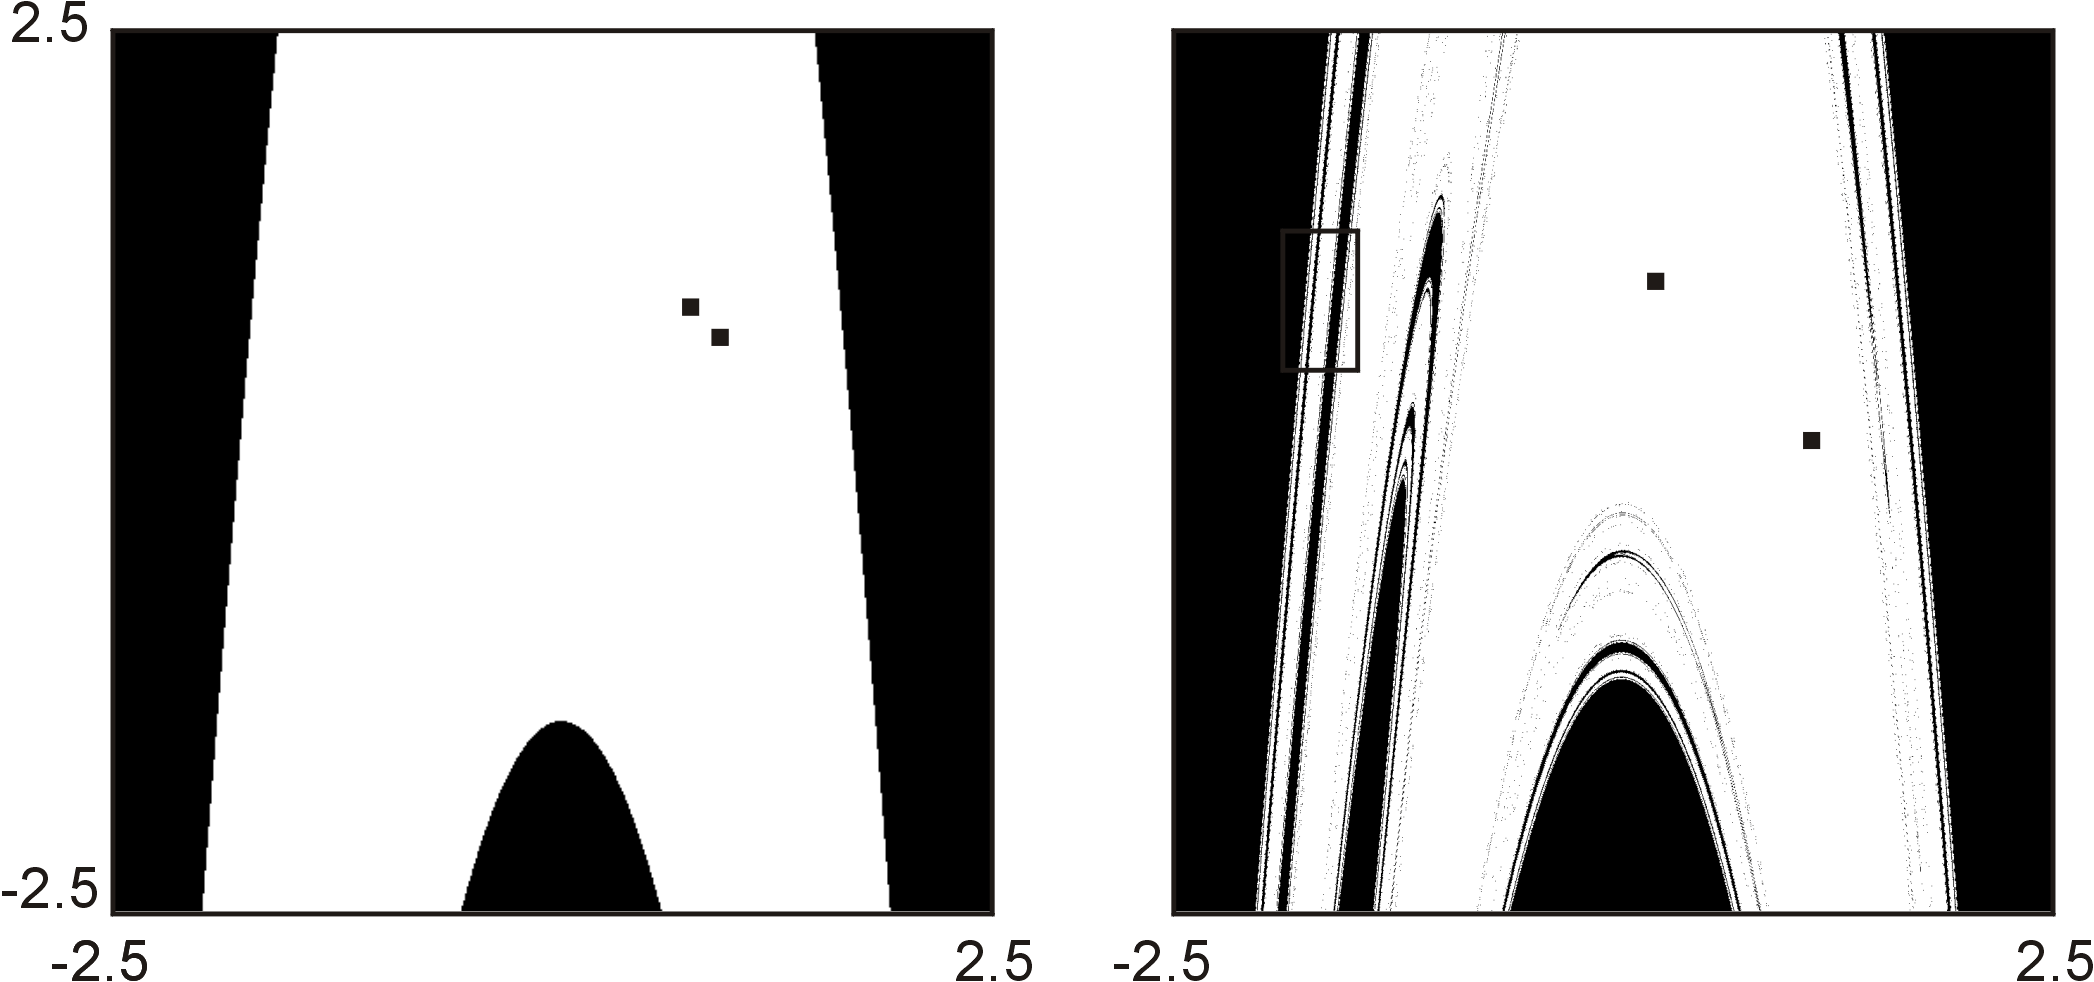
\includegraphics[width=11cm]{dynamic/figures/henon_basin}
\caption{Influence of initial conditions for the H\'{e}non map with $b=-0.3$. Initial values whose trajectories diverge to infinity are coloured black. The squares show the location of a period--2 sink, which attracts white initial conditions. On the left, $a=1.28$ and the basin boundary is smooth. On the right, $a=1.4$, and the boundary is fractal.}
\label{fig-henon-basin}
\end{figure} 

For $a=1.4$ and $b=-0.3$, we get a completely different picture: the boundary of the basin is no longer smooth, but is in a sense infinitely complicated: if we were to zoom in on it, we would still see the same level of complexity, no matter how deep we would zoom. This is illustrated in Fig.~\ref{fig-henon-zoom}, which shows successive zooms of a small region of the basin boundary, indicated by a rectangle in the picture. The \emph{self--similarity} at different zoom levels is apparent. We call such a self--similar structure with infinite complexity a \emph{fractal}.

\begin{figure}
\centering
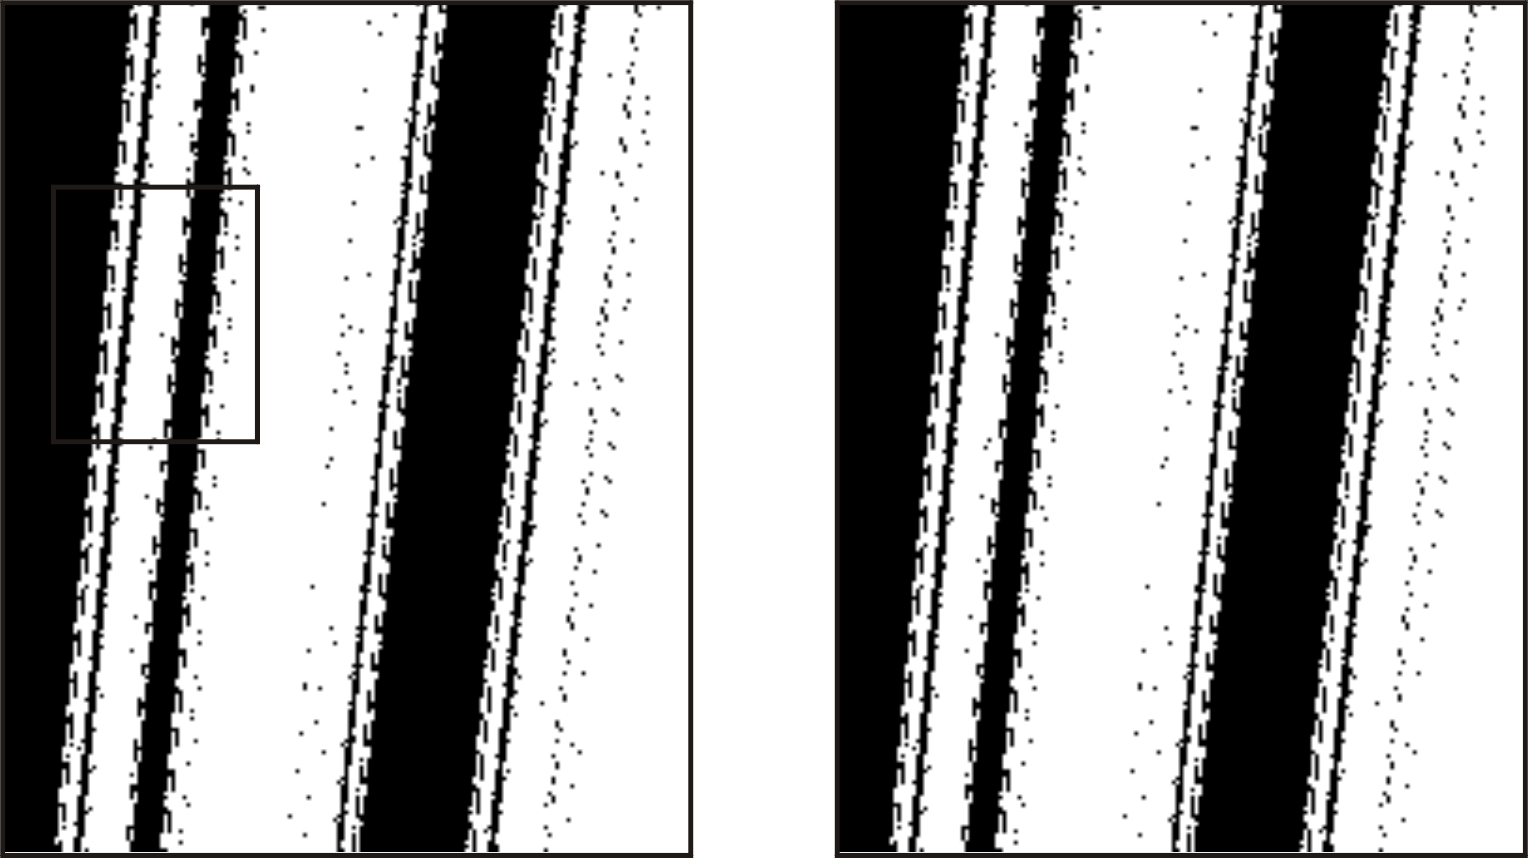
\includegraphics[width=8cm]{dynamic/figures/henon_zoom}
\caption{Self--similarity of the H\'{e}non basin boundary for $a=1.4$ and $b=-0.3$. The left picture corresponds to $[-1.88,-1.6] \times [-0.52,-0.24]$, which was indicated by the box in Fig.~~\ref{fig-henon-basin}. The right picture corresponds to the box in the left picture.}
\label{fig-henon-zoom}
\end{figure} 

Let us finally flip the sign of $b$ and look at the case $a=1.4$ and $b=0.3$. Now the period--2 sink disappears, and the orbit will eventually evolve to look like the structure in Fig.~\ref{fig-henon-attractor}. This is an example of a dynamical system with a \emph{fractal attractor}, as it turns out that this attractor is once again self--similar at different zoom levels. The orbit of nearly any point in this region will converge to this attractor. Note that this does not mean that two slightly different initial conditions will converge to the same limiting behaviour. In fact, the opposite is true: because of the infinitely complicated nature of the attractor, the two orbits will eventually diverge and become completely uncorrelated.

\begin{figure}
\centering
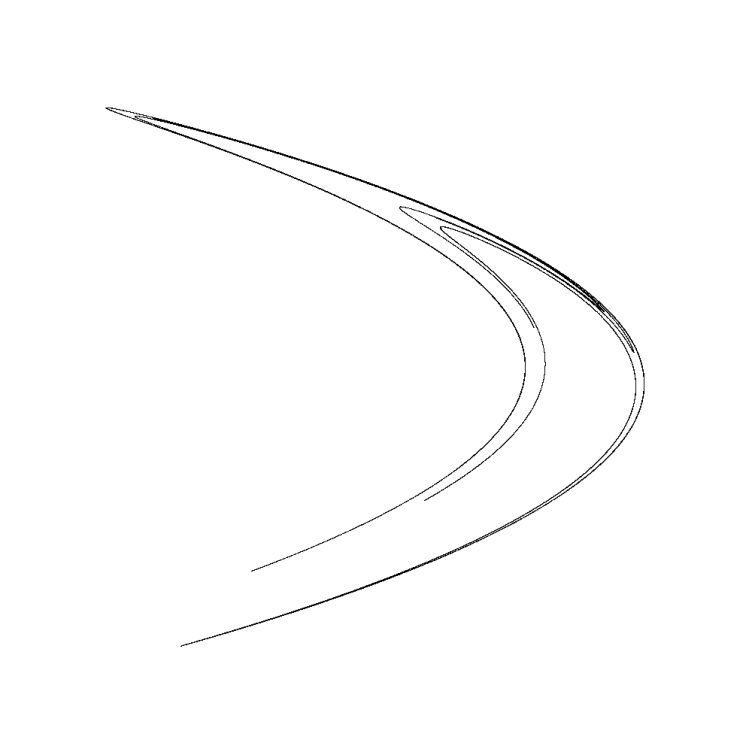
\includegraphics[width=8cm]{dynamic/figures/henon_attractor}
\caption{Plot of the H\'{e}non attractor in the $(x,y)$--plane for $a=1.4$ and $b=0.3$.}
\label{fig-henon-attractor}
\end{figure} 

\begin{sidebar}
\begin{ex}
Consider the following family of 2D maps, this time expressed in terms of a complex coordinate $z$:
$$P_c(z)=z^2+c$$
For each value of $c$, check numerically if the orbit of the initial point $z=0$ diverges towards infinity. Plot the points $c$ for which this orbit stays bounded. The set of these points is called the \emph{Mandelbrot set} and is plotted in Fig.~\ref{fig-mandelbrot}.
\end{ex}
\end{sidebar}

\begin{figure}
\centering
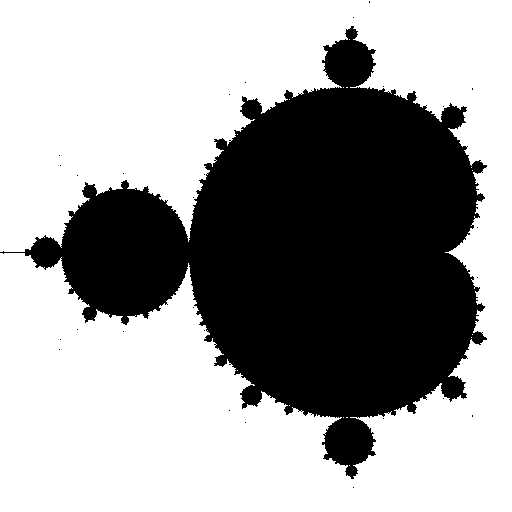
\includegraphics[width=8cm]{dynamic/figures/mandelbrot}
\caption{The Mandelbrot set.}
\label{fig-mandelbrot}
\end{figure} 

\begin{sidebar}
\begin{ex}
Show that the Mandelbrot set has mirror symmetry along the real axis.
\end{ex}
\end{sidebar}

\subsection{Saddle points}

We used the term 'sink' in our discussion of 1D maps to refer to a fixed point or a periodic orbit that attracts an epsilon neighbourhood of initial values. A 'source' is a fixed point that repels a neighbourhood. These definitions make sense in higher--dimensional state spaces without alteration. In 2D e.g., the neighbourhoods in question are disks.

Fig.~\ref{fig-circle-images} shows schematic views of a sink and a source for a 2D map, together with a typical disk neighbourhood and its image under the map. Along with the sink and the source, a new type of fixed point is introduced, which cannot occur in 1D systems. This type of point, which we call a \emph{saddle}, has at least one attracting direction and one repelling direction. 
\begin{figure}
\centering
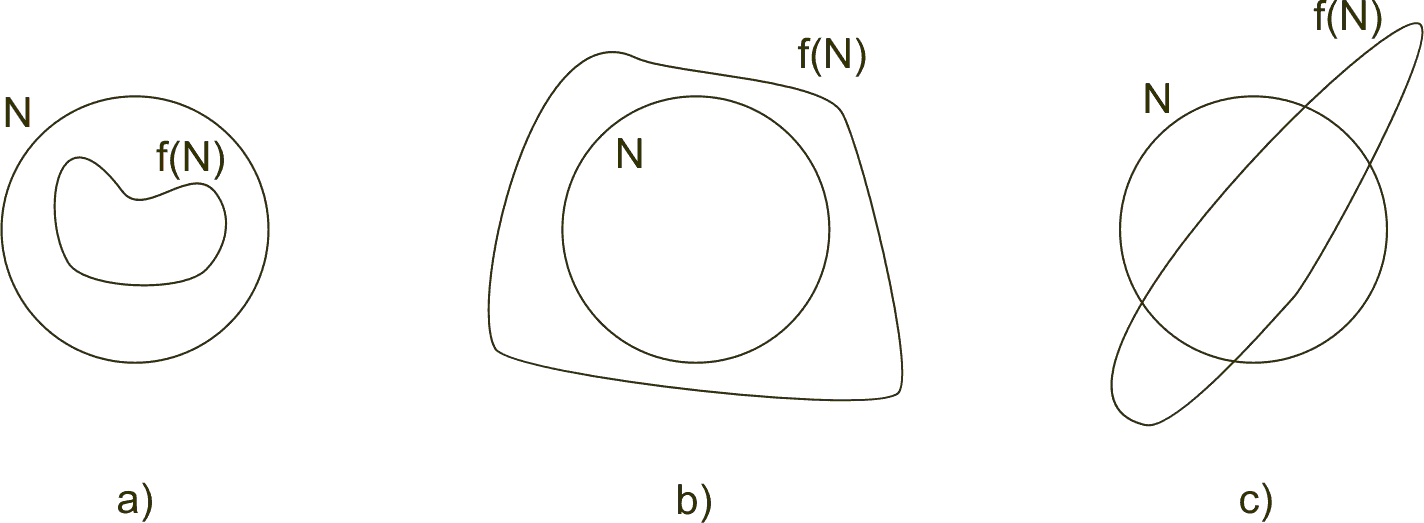
\includegraphics[width=12cm]{dynamic/figures/circle_images}
\caption{Images of a disk in the neighbourhood of a $a)$ sink, $b)$ source, $c)$ saddle point.}
\label{fig-circle-images}
\end{figure} 

Points near this type of fixed point act as if they were moving along the surface of a cowboy's saddle under the influence of gravity. This is illustrated in Fig.~\ref{fig-saddle}. A saddle exhibits sensitive dependence on initial conditions, because of the neighbouring initial conditions that escape along the repelling direction.

\begin{figure}
\centering
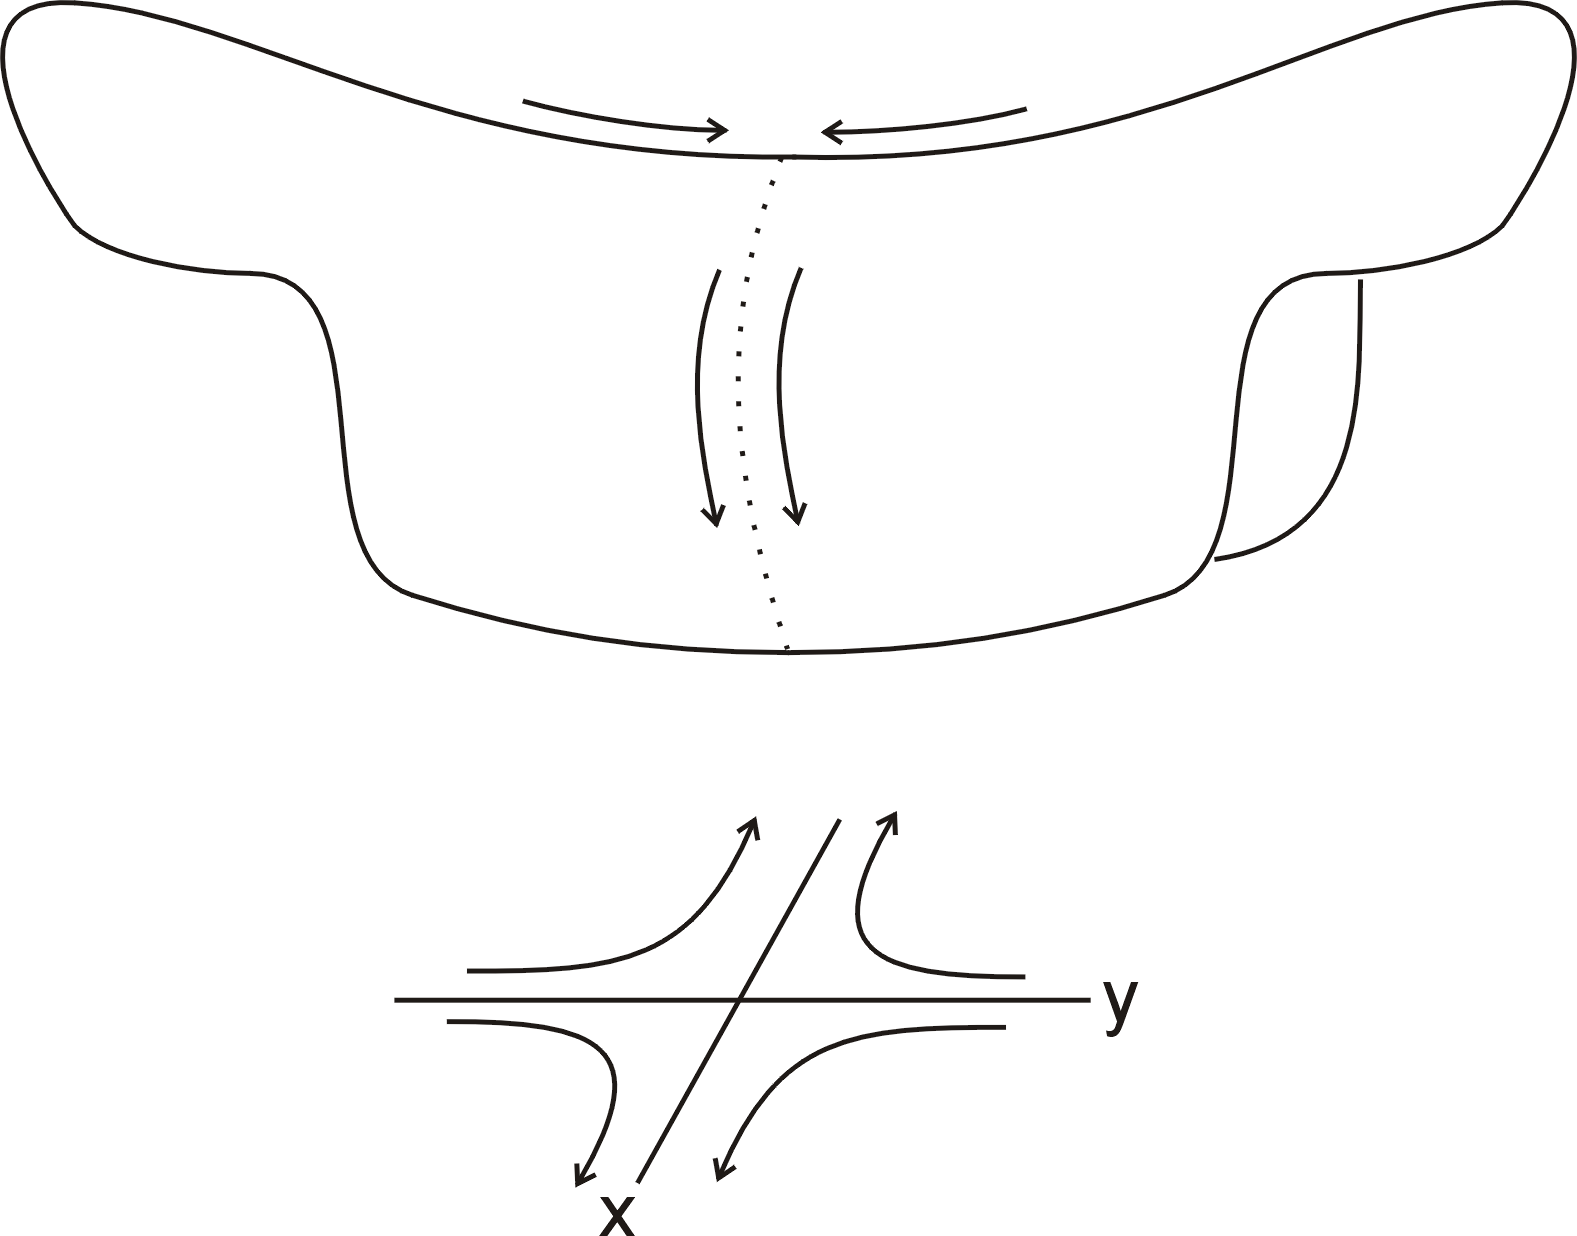
\includegraphics[width=7cm]{dynamic/figures/saddle}
\caption{A saddle point.}
\label{fig-saddle}
\end{figure} 

Saddle points play surprising roles in the dynamics of a system. To already give an example of this, let's return to Fig.~\ref{fig-henon-basin}, where black points are in the basin of infinity and white points are in the basin of sink. What happens to points which are located on the boundary between these two basins? Will they converge towards the sink or towards infinity? The answer is: neither. It turns out that these points converge towards the saddle! So, although not a general attractor, the saddle obviously plays an important role in determining which points go to which basin.

Our goal in the next sections is to find ways of identifying sources, sinks and saddles from the defining equations of the map. In 1D systems, we already saw that the key to determining stability was looking at the derivative in that point. Since the derivative determines the tangent line, or the best linear approximation near that point, it determines the amount of shrinking/stretching in the vicinity of that point. The same principle operates in higher dimensional systems, where we need to look at the best linear approximation of the system at that point. Before constructing such a linearisation, let's first study linear maps and see what we can learn from them.

\subsection{Linear maps}

A 2D linear map is described by a simple matrix multiplication:

\begin{gather}
f(x,y) = {\bf A} 
\begin{bmatrix}
x \\
y
\end{bmatrix}
=
\begin{bmatrix}
a_{11} & a_{12} \\
a_{21} & a_{22}
\end{bmatrix}
\begin{bmatrix}
x \\
y
\end{bmatrix}
\end{gather} 

Every linear map has a fixed point at the origin. Its stability can be investigated in the same way as we did for 1D maps: if all points in the neighbourhood of the fixed point approach the fixed point when iterated by the map, we consider the fixed point to be an attractor.

In some cases, the dynamics of a 2D system resemble 1D dynamics. This is the case when the initial point ${\bf v_0}$ is an eigenvector of ${\bf A}$ with eigenvalue $\lambda$. Then we get:

\begin{gather}
{\bf v_1} = {\bf A}{\bf v_0} = \lambda {\bf v_0} \\
{\bf v_2} = {\bf A}\lambda {\bf v_0} = \lambda^2 {\bf v_0} 
\end{gather} 

and in general ${\bf v_n} = \lambda^n {\bf v_0}$. Hence the map behaves like the 1D map $v_{n+1} = \lambda v_n$.

The importance of eigenvalues is further exemplified by looking at the orbit of an arbitrary point. Let's restrict ourselves for the moment to the case where the eigenvalues $\lambda_i$ of ${\bf A}$ are real and distinct, so that we can diagonalise the matrix as follows:

\begin{equation}
{\bf A} = {\bf S}^{-1}
\begin{bmatrix}
\lambda_{1} & 0 \\
0 & \lambda_{2}
\end{bmatrix} 
{\bf S}
\end{equation} 

Now, after $n$ iterations, the orbit of a starting vector ${\bf x}_0$ looks as follows:

\begin{equation}
{\bf x}_n = {\bf A}^n {\bf x}_0 = {\bf S}^{-1}
\begin{bmatrix}
\lambda_1^n & 0 \\
0 & \lambda_2^n
\end{bmatrix} 
{\bf S} {\bf x}_0 
\end{equation} 

From this, we see immediately that if all eigenvalues have a magnitude smaller than 1, the orbit converges to our fixed point $(0,0)$. On the other hand, if all eigenvalues have a magnitude larger than 1, the iterates will diverge, meaning that the fixed point is unstable. Finally, for one eigenvalue smaller than 1, and one eigenvalue larger than 1, we have saddle point, as there is one converging and one diverging direction.

Obviously, not all $2 \times 2$ matrices can be diagonalised. We know from linear algebra that there are two other canonical forms for $2 \times 2$ matrices. E.g., when the eigenvalues are not distinct, the canonical form is
\begin{equation}
{\bf A} = 
{\bf S}^{-1}
\begin{bmatrix}
\lambda_1 & 1 \\
0 & \lambda_1
\end{bmatrix} 
{\bf S}
\end{equation} 

When the eigenvalues are a complex conjugate pair, the matrix can be diagonalised using complex numbers. However, one can prove that another, more useful \emph{real} canonical form of such a matrix exists, namely:

\begin{equation}
{\bf A} = 
{\bf S}^{-1}
\begin{bmatrix}
a & -b \\
b & a
\end{bmatrix} 
{\bf S}
\end{equation} 

\begin{sidebar}
\begin{ex}
Show that for these other canonical forms, the same conclusions with respect to stability of the fixed point at the origin hold as in the case of real distinct eigenvalues.
\end{ex}
\end{sidebar}

\begin{sidebar}
\begin{ex}
For the following maps, determine whether the origin is a sink, source or saddle.

a) $$\begin{bmatrix}4 & 30 \\ 1 & 3 \end{bmatrix}$$

b) $$\begin{bmatrix}1 & 1/2 \\ 1/4 & 3/4 \end{bmatrix}$$

\end{ex}
\end{sidebar}

\begin{sidebar}
\begin{ex}
Find

$$\lim_{n \to \infty}\begin{bmatrix}4.5 & 8 \\ -2 & -3.5 \end{bmatrix} ^ n \begin{bmatrix} 6 \\ 9 \end{bmatrix}$$

\end{ex}
\end{sidebar}

\subsection{Nonlinear maps and the Jacobian matrix}

To construct the linearisation around a fixed point, we now have to calculate a matrix rather than a single derivative. This matrix is called the \emph{Jacobian} and is defined as follows.

Let ${\bf f}=(f_1,f_2, ... ,f_n)$ be a map on $\mathbb{R}^n$ and let ${\bf p} \in \mathbb{R}^n$. The Jacobian matrix of ${\bf f}$ at ${\bf p}$, denoted as ${\bf Df}({\bf p})$, is defined as

\begin{equation}
{\bf Df}({\bf p})=
\begin{bmatrix}
\frac{\partial f_1}{\partial x_1}({\bf p}) & \cdots & \frac{\partial f_1}{\partial x_n}({\bf p}) \\
\vdots & & \vdots \\
\frac{\partial f_n}{\partial x_1}({\bf p}) & \cdots & \frac{\partial f_n}{\partial x_n}({\bf p}) \\
\end{bmatrix} 
\end{equation} 

Given a vector ${\bf p}$ and a small increment {\bf h}, the increment in ${\bf f}$ due to ${\bf h}$ is given by

\begin{equation}
{\bf f}({\bf p} + {\bf h}) - {\bf f}({\bf p}) = {\bf Df}({\bf p}) \cdot {\bf h} + O\left(|{\bf h}|^2\right)
\end{equation} 

For a fixed point, ${\bf f}({\bf p}) = {\bf p}$, so for a small change ${\bf h}$, the map moves ${\bf p} + {\bf h}$ approximately ${\bf Df}({\bf p}) \cdot {\bf h}$ away from ${\bf p}$. That is, ${\bf f}$ magnifies a small change ${\bf h}$ in input to a change ${\bf Df}({\bf p}) \cdot {\bf h}$ in output.

As long as this deviation remains small (so that $|{\bf h}|^2$ is negligible and our approximation is valid), the action of the map near ${\bf p}$ is essentially the same as the linear map ${\bf A} = {\bf Df}({\bf p})$, with fixed point ${\bf h} = 0$. So, we can use our stability criteria for linear maps we have discussed so far.

Although we won't prove it here, in the general case of $n$--dimensional maps, the following stability criteria hold:

Let ${\bf f}$ be a map on $\mathbb{R}^n$ and assume ${\bf f}({\bf p})={\bf p}$.

\begin{enumerate}
\item
If the magnitude of each eigenvalue of ${\bf Df}({\bf p})$ is less than 1, then ${\bf p}$ is a sink.
\item
If the magnitude of each eigenvalue of ${\bf Df}({\bf p})$ is greater than 1, then ${\bf p}$ is a source.
\item
If none of the eigenvalues of ${\bf Df}({\bf p})$ has magnitude equal to 1 (we call ${\bf p}$ \emph{hyperbolic} then), if at least one eigenvalue of ${\bf Df}({\bf p})$ has magnitude less than 1, and at least one eigenvalue of ${\bf Df}({\bf p})$ has magnitude greater than 1, then ${\bf p}$ is a saddle.
\end{enumerate}

\begin{sidebar}
\begin{ex}
Consider the map 

$$f(x,y) = (-x^2+0.4y, x)$$

Discuss the stability of the fixed points $(0,0)$ and $(-0.6,-0.6)$.

\end{ex}
\end{sidebar}

\begin{sidebar}
\begin{ex}
% Source: Chaos - Alligood
Consider the map 

$$f(x,y) = (x^2-5x+y, x^2)$$

Find the fixed points and discuss their stability.

\end{ex}
\end{sidebar}

\begin{sidebar}
\begin{ex}
Consider the linear map defined as $f(x,y) = (2x+y, x+y)$ with a corresponding matrix $A$. Discuss the stability of its fixed point.\\

Now, consider the nonlinear map defined as $g(x,y) = (2x+y, x+y)\, mod \, 1$, i.e. the same update rule as above but with an added modulo 1 operator. Show that $(1/3, 1/3)$ is a periodic point with period 4 of this nonlinear map.\\

Next, discuss the stability of this periodic point.\\

\textit{Hint}: the modulo operator can be applied after several updates and will lead to the same result, e.g.  $g(g(x,y)) = f(f(x,y)) \, mod \, 1$ (no need to prove this).\\
\textit{Hint 2}: consider $A^4 \begin{bmatrix} 1/3 + \delta_x \\ 1/3 + \delta_y \end{bmatrix} \, mod \, 1$ and looks what happens to the perturbation, without calculating any new eigenvalues, but using what you've determined about the stability of the fixed point of $A$.\\

Finally, you just showed that the point $(1/3, 1/3)$ is a periodic point, yet if we compute its evolution numerically we obtain a chaotic behaviour. Explain why.
\end{ex}
\end{sidebar}


\subsection{Stable and unstable manifolds}

Without providing any proofs, we will discuss in this section some more aspects of the special properties of saddle points.

We have seen that a saddle point is unstable, in the sense that most initial conditions will move away from it because the existence of an expanding direction. However, not all initial conditions will move away. Consider e.g. this very simple linear map:

\begin{equation}
A =
\begin{bmatrix}
0.9 & 0 \\
0 & 1.1
\end{bmatrix} 
\label{eq-map-ex}
\end{equation} 

For initial values on the $x$--axis, the orbit will converge to the saddle point, because it does not feel the influence of the expanding direction. This set of points is important enough to warrant its own name:

The \emph{stable manifold} of a saddle point ${\bf p}$ is defined as the set of points ${\bf v}$ for which $|{\bf f}^n({\bf v}) - {\bf p} | \to 0$ as $ n \to \infty$.

For 2D maps, one can prove the following properties about the stable manifold. First of all, it is one--dimensional \footnote{A one--dimensional manifold is a set of points that locally looks like a line everywhere along its length. E.g. the letter 'O' is a 1--manifold. The letter 'T' on the other hand is not, because of the intersection and the end points.}. Secondly, the stable manifold will be tangent to the eigenvector of the matrix ${\bf Df}({\bf p})$ with eigenvalue smaller than 1.

In the example from Eq.~\ref{eq-map-ex}, the $y$--axis is the \emph{unstable manifold} of the saddle point. It is defined as follows:

The unstable manifold of a saddle point ${\bf p}$ is defined as the set of points ${\bf v}$ for which $|{\bf f}^{-n}({\bf v}) - {\bf p}| \to 0$ as $ n \to \infty$, so points in the unstable manifold converge to the saddle point when iterating the map backwards. In other words, the unstable manifold is the stable manifold of the inverse map ${\bf f}^{-1}$.

Note that we have not defined the unstable manifold as the set of points for which $|{\bf f}^{n}({\bf v}) - {\bf p}| \to \infty$, as this would be too restrictive. There are points on the unstable manifold which diverge to infinity under the forward maps, but there are also points which get trapped in a chaotic orbit.

For the unstable manifold, similar properties hold as for the stable manifold. It is a 1--manifold, and it is tangent to eigenvector of the Jacobian with eigenvalue larger than 1.

For linear maps, the stable and unstable manifolds are easily determined, and are just lines in the direction of the eigenvectors of the Jacobian. For nonlinear maps, they can look significantly more complicated, as is illustrated in Fig.~\ref{fig-manifold} for a H\'{e}non map. 

\begin{figure}
\centering
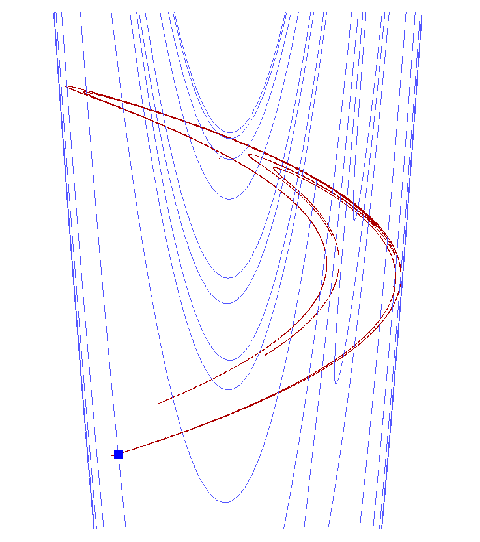
\includegraphics[width=7cm]{dynamic/figures/manifold}
\caption{Stable and unstable manifold of a H\'{e}non map. The saddle point is the square in the lower left corner, the stable manifold is mainly vertical, the unstable one mainly horizontal.}
\label{fig-manifold}
\end{figure} 

The shape of these curves should look familiar. Indeed, the following properties hold:

\begin{enumerate}
\item
The stable manifold forms the boundary between the basin of the sink and the basin at infinity.
\item
The attractor of the map lies along the unstable manifold (which can be either a periodic sink, or a chaotic attractor)
\end{enumerate}

A further important aspect of the unstable and stable manifold is the following: if they cross (at another point than the saddle of course), there are automatically an infinite numbers of such crossings. Also, the system will show chaotic behaviour in such a case.

These insights are mainly due to Poincar\'{e}, who developed much of the theory underlying chaotic systems when studying the dynamics of three bodies moving under the force of gravity.
 
\section{Continuous systems}

\subsection{Relation with discrete maps}

In the last part of this chapter, we will discuss some introductory concepts on continuous dynamical systems, i.e. those that are described by differential equations rather than difference equations.

Since we have already spent so much time discussing discrete maps, it would be nice to have some tools to reduce a continuous system to a discrete one and be able to study some aspects of its dynamics in that way. There are two methods that can be used for this: the time--$T$ map and the Poincar\'{e} map.

A \emph{time--$T$ map} is formed by taking snapshots at fixed time intervals of the solution of the continuous system, i.e. a time--$T$ map is a discrete map that advances the continuous system $T$ time units. 

Sometimes it is possible to write down an explicit equation for a time--$T$ map. Consider e.g. the differential equation which describes the cooling of an object with specific heat $k$:

\begin{equation}
\frac{dx}{dt} = -k x
\end{equation} 

Here $x$ stands for temperature. The solutions of this equation are of the form

\begin{equation}
x(t) = x_0 e^{-kt}
\end{equation} 

Advancing from time $t_0$ to $t_0+T$ amounts to a multiplication with $e^{-kT}$. So, the time--$T$ map for this system is the 1D map with the following update function:

\begin{equation}
f(x) = e^{-kT} x
\end{equation} 

If it's not possible to write down an explicit rule, then the map has to be iterated numerically.

Note that the laser dynamics example from the opening of the chapter also used the time--$T$ philosophy, as the system was studied at specific snapshots in time determined by the sampling frequency.

Another technique to reduce a continuous system to a discrete one is the so--called \emph{Poincar\'{e} map}. One of Poincar\'{e}'s most important innovations was a simplified way of looking at complex continuous trajectories. Instead of studying the entire trajectory, he found that much of the important information was encoded in the points at which the trajectory passes through a two--dimensional plane. The order of these intersection points defines a discrete plane map, which is called the Poincar\'{e} map. 

Fig.~\ref{fig-poincare} shows a schematic view of a trajectory $C$. The plane $S$ is defined by $x_3=$ constant. Each time the trajectory $C$ pierces $S$ in a downward direction, as at points ${\bf A}$ and ${\bf B}$, we record the point of piercing on the plane $S$. We can label these points with coordinates $(x_1,x_2)$. Let ${\bf A}$ represent the $k$--th downward piercing of the plane, and ${\bf B}$ the $(k+1)$--th downward piercing. The Poincar\'{e} map is the 2D map $G$ such that $G({\bf A}) = {\bf B}$.

\begin{figure}
\centering
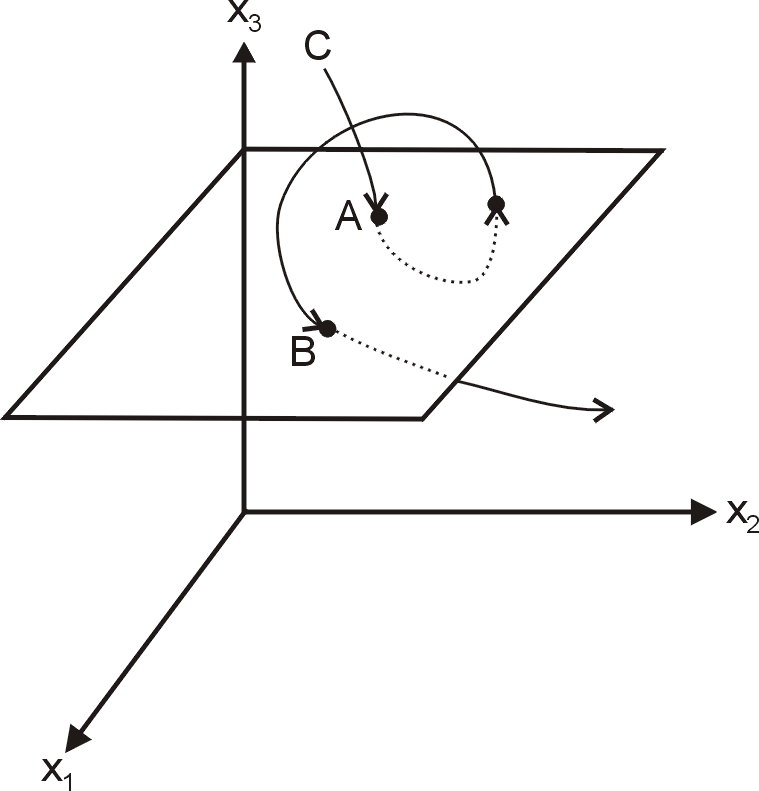
\includegraphics[width=6cm]{dynamic/figures/poincare}
\caption{Poincar\'{e} map of a trajectory.}
\label{fig-poincare}
\end{figure} 

Given ${\bf A}$, the differential equations can be solved with ${\bf A}$ as initial condition, and the solution followed until the next downward piercing at ${\bf B}$. Thus ${\bf A}$ uniquely determines ${\bf B}$, which ensures that the map $G$ is well--defined. Much of the dynamical behaviour of the trajectory $C$ is present in the 2D map $G$. E.g, if $C$ is periodic in the sense that it follows a closed loop, then the plane map $G$ will have a periodic orbit.

The Poincar\'{e} map is similar in principle to the time--$T$ map we considered above, although the details are different. While the time--$T$ map is stroboscopic (it logs the value of a variable at equal time intervals), the Poincar\'{e} map records plane piercings, which need not be equally spaced in time.

\subsection{Phase portraits}

If we do want to study the trajectory $C$ without reducing it to a discrete map, it is often useful to construct phase portraits (also called phase planes) of the solutions of a differential equation. 

To illustrate what these are, let's return to the simple differential equation

\begin{equation}
\frac{dx}{dt} = -k x
\end{equation} 

with solutions

\begin{equation}
x(t) = x_0 e^{-kt}
\end{equation} 

\begin{figure}
\centering
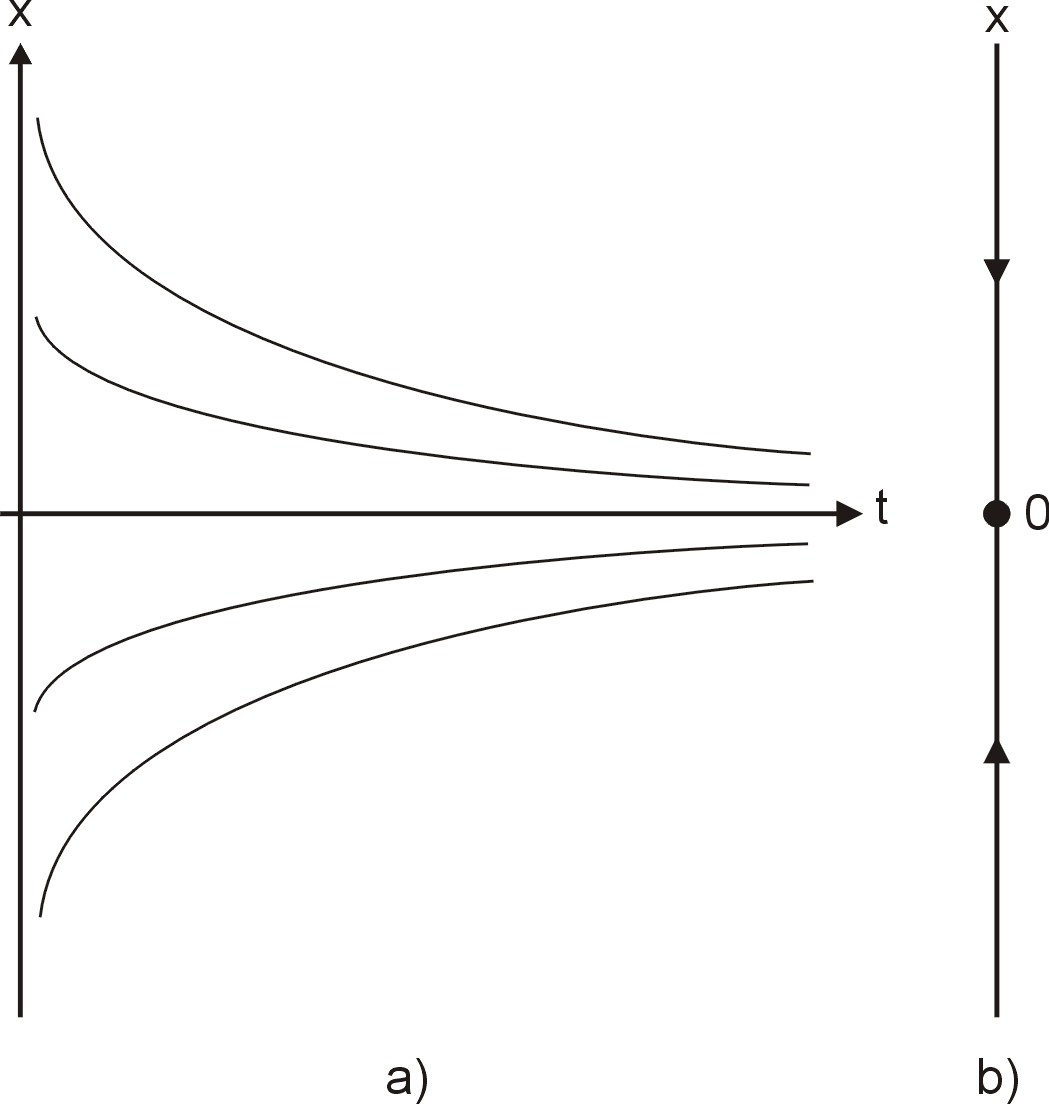
\includegraphics[width=6cm]{dynamic/figures/phaseportrait}
\caption{$a)$ Solutions of ${dx}/{dt} = -k x$ for different initial conditions. $b)$ Corresponding phase portrait.}
\label{fig-phaseportrait}
\end{figure} 

Fig.~\ref{fig-phaseportrait} a) sketches several trajectories of $x$ for different initial values. All curves converge to the equilibrium value $x=0$. An \emph{equilibrium} solution is a solution of the differential equation which satisfies $dx/dt = 0$. They play the same role as fixed points in discrete maps, and are therefore important to study.

Often, a figure like Fig.~\ref{fig-phaseportrait}  a) contains too much information, as we are often only interested in the stability of the equilibrium. We are not so much interested in the different curves for different initial conditions, nor in the precise rate at which the equilibrium is approached. This leads to the \emph{phase portrait} in Fig.~\ref{fig-phaseportrait} b), in which the $t$--axis is suppressed, and it is simply shown on the $x$--axis where trajectories are headed. The arrows indicate the direction of solutions (towards or away from equilibria) without graphing specific values of $t$. The phase portrait allows one to see at a glance where the equilibria are located and whether they are stable or not.

\begin{sidebar}
\begin{ex}
Construct a phase portrait for the logistic differential equation:
$$\frac{dx}{dt} = a x (1-x)$$
\end{ex}
\end{sidebar}

\subsection{The Lorenz attractor}

We finish the chapter by looking at the most famous set of differential equations which exhibit chaotic behaviour. They were formulated in the early 1960s by Lorenz, in the context of weather forecasting:

\begin{align}
\frac{dx}{dt} =& -\sigma x + \sigma y \\
\frac{dy}{dt} =& -xz + r y - y \\
\frac{dz}{dt} =& xy - bz
\end{align} 

For $\sigma=10$ and $b=8/3$, Lorenz found that the system behaves 'chaotically' whenever $r$ exceeds the critical value of $24.74$. In that case, all solutions appear to be extremely sensitive to initial conditions, and almost all of them are apparently neither periodic solutions nor convergent to periodic solutions or equilibria. Instead, he found found one of the very first chaotic attractors, which is now called the Lorenz attractor. This attractor is plotted in Fig.~\ref{fig-lorenz}.

\begin{figure}
\centering
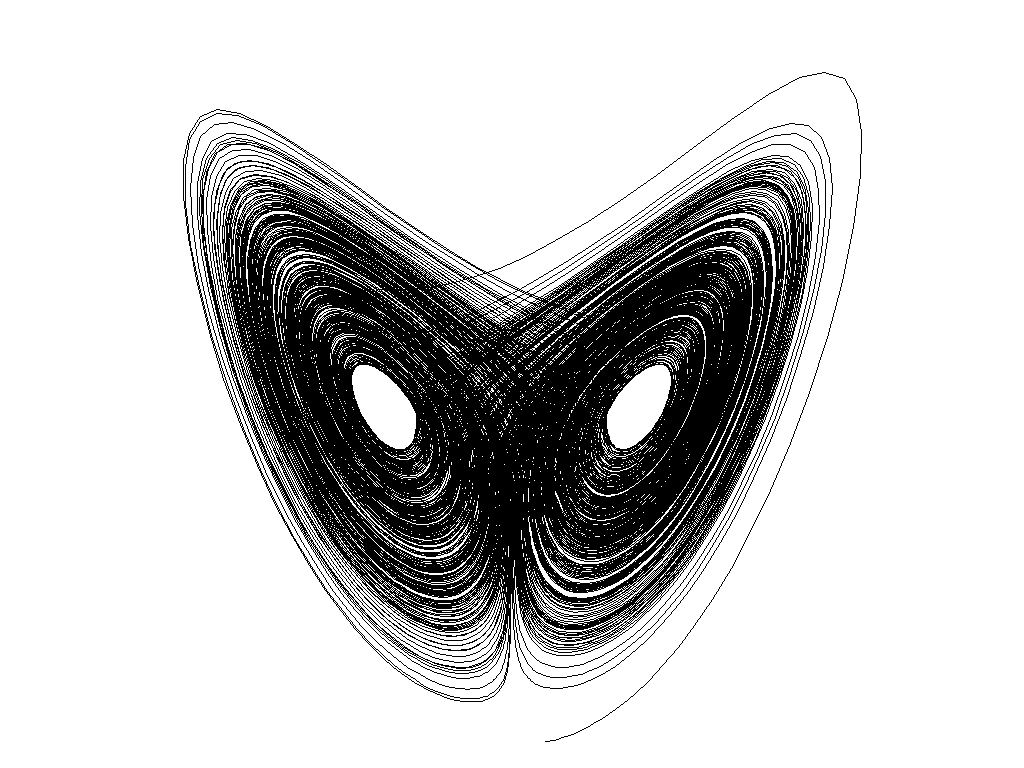
\includegraphics[width=10cm]{dynamic/figures/lorenz}
\caption{The Lorenz attractor.}
\label{fig-lorenz}
\end{figure} 


Lorenz realised that this sensitivity on initial conditions has a huge impact on weather predicting. In fact, the title of one of his talks was: "Predictability: Does the Flap of a Butterfly's Wings in Brazil set off a Tornado in Texas?". This is why sensitivity on initial conditions is sometimes referred to as 'the butterfly effect'.

\pagebreak

\section*{Jules Henri Poincar\'{e} (1854--1912)}

\parpic{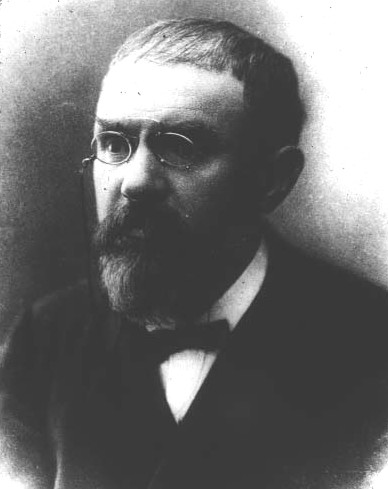
\includegraphics[scale=0.5]{dynamic/figures/poincare_photo}}

Jules Henri Poincar\'{e} was born in 1854 in Nancy, a city in France. In 1862 Henri entered the Lyc\'{e}e of Nancy which is today, called in his honor, the Lyc\'{e}e Henri Poincar\'{e}. In fact the University of Nancy is also named in his honour. He graduated from the Lyc\'{e}e in 1871 with a bachelors degree in letters and sciences. Henri was the top of class in almost all subjects, he did not have much success in music and was described as 'average at best' in any physical activities. This could be blamed on his poor eyesight and absentmindedness. Later in 1873, Poincar\'{e} entered l'Ecole Polytechnique where he performed better in mathematics than all the other students. He published his first paper at 20 years of age and graduated from the institution in 1876. The same year he decided to attend l'Ecole des Mines and graduated in 1879 with a degree in mining engineering. After his graduation he was appointed as an ordinary engineer in charge of the mining services in Vesoul. At the same time he was preparing for his doctorate in sciences (not surprisingly), in mathematics under the supervision of Charles Hermite. Poincar\'{e}, as expected graduated from the University of Paris in 1879, with a thesis relating to differential equations. He then became a teacher at the University of Caen, where he taught analysis. He remained there until 1881. He then was appointed as the professor in charge of analysis courses at the University of Paris. Also in that same year he married Miss Poulain d'Andecy. He had now returned to work at the Ministry of Public Services as an engineer, responsible for the development of the northern railway. This was the last job he held in administration for the government of France. In 1893 he was awarded the title of head engineer in charge of the mines. After that his career awards and position continuously escalated in greatness and quantity. He died two years before the war on July 1912 of an embolism at the age of 58. Interestingly, at the beginning of World War I, his cousin Raymond Poincar\'{e} was the president of the French Republic.

Poincar\'{e}'s work habits have been compared to a bee flying from flower to flower. Poincar\'{e} was interested in the way his mind worked, he studied his habits. He linked his way of thinking to how he made several discoveries. He worked during the same times each day in short periods of time. He never spent a long time on a problem since he believed that the subconscious would continue working on the problem while he worked on another problem. 

The mathematician Darboux claimed he was \emph{un intuitif}, arguing that this is demonstrated by the fact that he worked so often by visual representation. Poincar\'{e} did not care about being rigorous and disliked logic. He believed that logic was not a way to invent but a way to structure ideas and that logic limits ideas. 

Poincar\'{e}'s first area of interest in mathematics was the Fuchsian function that he named after the mathematician Lazarus Fuch because Fuch was known for being a good teacher and done alot of research in differential equations and in the theory of functions. The functions did not keep the name fuchsian and are today called automorphic. Poincar\'{e} actually developed the concept of those functions as part of his doctoral thesis. Below Poincar\'{e} explains how he discovered Fuchsian functions:

For fifteen days I strove to prove that there could not be any functions like those I have since called Fuchsian functions. I was then very ignorant; every day I seated myself at my work table, stayed an hour or two, tried a great number of combinations and reached no results. One evening, contrary to my custom, I drank black coffee and could not sleep. Ideas rose in crowds; I felt them collide until pairs interlocked, so to speak, making a stable combination. By the next morning I had established the existence of a class of Fuchsian functions, those which come from the hypergeometric series; I had only to write out the results, which took but a few hours. 

In 1887, Oscar II, King of Sweden and Norway held a competition to celebrate his sixtieth birthday and to promote higher learning. The King wanted a contest that would be of interest so he decided to hold a mathematics competition. Poincar\'{e} entered the competition submitting a memoir on the three body problem which he describes as:

The goal of celestial mechanics is to answer the great question of whether Newtonian mechanics explains all astronomical phenomenons. The only way one can prove this is by taking the most precise observation and comparing it to the theoretical calculations.

Poincar\'{e} did in fact win the competition. In his memoir he described new mathematical ideas such as homoclinic points (the intersections between the stable and unstable manifolds of the same saddle point). The memoir was about to be published in Acta Mathematica when an error was found by the editor. This error in fact led to the discovery of chaos theory. The memoir was published later in 1890. In addition Poincar\'{e} proved that the determinism and predictability were disjoint problems. He also found that the solution of the three body problem would change drastically with small change on the initial conditions. This area of research was neglected until 1963 when Edward Lorenz discovered the famous a chaotic deterministic system using a simple model of the atmosphere.

Henri Poincar\'{e} and Albert Einstein had an interesting relationship concerning their work on relativity. Their interaction begins in 1905 when Poincar\'{e} published his first paper on relativity. About a month later Einstein published his first paper on relativity. Both continued publishing work about relativity, but neither of them would reference each others work. Not only did Einstein not reference Poincar\'{e}'s work but claimed never to have read it. On one occasion Einstein referenced Poincar\'{e} acknowledging his work on relativity in the text of a lecture in 1921. Although later in Einstein's life, he would comment on Poincar\'{e} as being one of the pioneers of relativity.

Poincar\'{e} made many contributions to different fields of applied mathematics such as: celestial mechanics, fluid mechanics, optics, electricity, telegraphy, capillarity, elasticity, thermodynamics, potential theory, quantum theory, theory of relativity and cosmology. In the field of differential equations Poincar\'{e} has given many results that are critical for the qualitative theory of differential equations, for example the Poincar\'{e} sphere and the Poincar\'{e} map.

It is that intuition that led him to discover and study so many areas of science. Poincar\'{e} is considered to be the next universalist after Gauss. After Gauss's death in 1855 people generally believed that there would be no one else that could master all branches of mathematics. However they were wrong because Poincar\'{e} took all areas of mathematics as 'his province'.

(after http://planetmath.org/encyclopedia/JulesHenriPoincare.html)
